\documentclass[12pt,a4paper]{article}

%% ── Packages ──────────────────────────────────────────────────────────────
\usepackage[a4paper, margin=2.5cm]{geometry}
\usepackage{amsmath,amssymb,amsfonts}
\usepackage{graphicx}
\usepackage{booktabs}
\usepackage{array}
\usepackage{tabularx}
\usepackage{longtable}
\usepackage{multirow}
\usepackage{hyperref}
\usepackage{setspace}
\usepackage{newunicodechar}
\newunicodechar{₂}{$_2$}
\usepackage{parskip}
\usepackage{enumitem}
\usepackage{caption}
\usepackage{subcaption}
\usepackage{float}
\usepackage[patch=none]{microtype}
\usepackage{algorithm}
\usepackage{algpseudocode}
\usepackage{mathtools}
\usepackage{bm}
\usepackage{titlesec}
\usepackage{fancyhdr}
\setlength{\headheight}{15pt}
\usepackage[T1]{fontenc}
\usepackage[utf8]{inputenc}

\hypersetup{colorlinks=false, hidelinks,
  pdftitle={Multi-Objective Quantum-Chemical MOF Recommendation},
  pdfauthor={}}

\onehalfspacing
\setlength{\parindent}{0pt}
\setlength{\parskip}{6pt}

\titleformat{\section}{\large\bfseries}{\thesection}{1em}{}
\titleformat{\subsection}{\normalsize\bfseries}{\thesubsection}{1em}{}
\titleformat{\subsubsection}{\normalsize\bfseries}{\thesubsubsection}{1em}{}

\captionsetup{font=small,labelfont=bf,format=plain,justification=justified}

\pagestyle{fancy}
\fancyhf{}
\fancyhead[L]{\small\textit{QMOF-Rec: Multi-Objective MOF Recommendation}}
\fancyhead[R]{\small\thepage}
\renewcommand{\headrulewidth}{0.4pt}

\newcolumntype{L}[1]{>{\raggedright\arraybackslash}p{#1}}
\newcolumntype{C}[1]{>{\centering\arraybackslash}p{#1}}
\newcolumntype{R}[1]{>{\raggedleft\arraybackslash}p{#1}}

\begin{document}

%% ── Title ─────────────────────────────────────────────────────────────────
\hypersetup{pageanchor=false}
\begin{titlepage}
\centering\vspace*{1cm}
{\LARGE\bfseries QMOF-Rec: A Multi-Objective Recommender-System Framework for Quantum-Chemical MOF Candidate Screening\par}
\vspace{2cm}
\begin{abstract}
\noindent
Large quantum-chemical materials databases require methods that rank candidates under competing objectives, incomplete descriptors, and application-specific user intent. We present QMOF-Rec, a query-driven recommender framework that formulates metal--organic framework (MOF) screening as a multi-objective top-$K$ ranking problem. The framework combines retrieval-based candidate generation with Lotus Effect Algorithm (LEA)-guided reranking, deterministic ranking baselines, formula-derived metadata-graph signals, and retrieval-augmented generation for scientific explanation.

The final diversity-aware, mask-aware protocol was rerun on 20{,}372 QMOF metadata records across five query scenarios, ten random seeds, and shared candidate pools. Density is available for all records, band gap for 10{,}810 records, and void fraction for none, so porosity is excluded from numerical ranking. A diagnosis showed that zero diversity in the prior mask-aware rerun was caused by binned utility scores, not identical raw materials. Diversity is therefore reported over a full-precision hybrid material representation combining observed density and band gap with formula- and graph-derived features. WeightedSum, TOPSIS, MMR, and baseline LEA tie on Rel@5 = 0.8479 and NDCG@5 = 1.0000. The LEA pipeline produced diversity of 0.0224 compared with 0.0187 for WeightedSum, while MMR reached 0.0241 at greater runtime; ablations did not isolate a measurable benefit from the explicit diversity or self-cleaning components. A 30-query deterministic candidate-conditioned explanation evaluation achieved full automated scores for grounding, metadata consistency, and limitation awareness, with no unsupported-claim flags. QMOF-Rec supports computational candidate prioritization and explanation, but no experimental, adsorption, or DFT validation is claimed.



\medskip\noindent\textbf{Keywords:}~QMOF, metal--organic frameworks, materials recommendation, multi-objective optimization, Lotus Effect Algorithm, retrieval-augmented generation, graph neural networks, GraphSAGE, graph attention networks, materials informatics, explainable AI
\end{abstract}
\end{titlepage}
\hypersetup{pageanchor=true}

%% ════════════════════════════════════════════════════════════════════════════
\section{Introduction}
\label{sec:intro}

Materials discovery increasingly depends on computational screening, machine learning, and interactive decision support because experimentally accessible materials spaces are too large to explore by manual intuition alone. Metal--organic frameworks (MOFs) are a representative example: their modular chemistry, tunable pore environments, and broad electronic-property landscape make them attractive for gas adsorption, storage, catalysis, separations, sensing, drug delivery, and electronic applications. Yet the same chemical diversity creates a practical recommendation problem.

We present QMOF-Rec, a multi-objective scientific recommender system for quantum-chemical MOF discovery. QMOF discovery can be formulated as a scientific top-$K$ recommendation task: given a user query and an incomplete set of material descriptors, the system must return a ranked and diverse shortlist of candidate MOFs that are relevant, scientifically plausible, and useful for follow-up investigation.

In this manuscript, \emph{quantum-chemical MOF recommendation} means recommending experimentally derived QMOF records using query intent together with available quantum-chemical and metadata-derived signals such as band gap, density, stability proxies, and graph-aware material relationships. The formulation extends conventional single-target screening by modelling recommendation as a multi-objective ranking problem over relevance, property suitability, diversity, and graph-aware material relationships.

The Quantum MOF (QMOF) database introduced by Rosen et al.\ provides quantum-chemical properties for experimentally derived MOF structures and has become an important resource for machine-learning-assisted MOF discovery \cite{rosen2021,rosen2022}. However, using QMOF as a recommendation substrate is different from using it as a static table. A scientific recommender must interpret user intent, retrieve a candidate pool, score property suitability, avoid redundant candidates, explain trade-offs, and communicate uncertainty when descriptors are missing. This is especially important for queries such as ``CO$_2$ adsorption MOFs'' or ``photocatalytic MOFs'', where semantic relevance alone is not equivalent to scientific suitability.

QMOF recommendation is a query-conditioned candidate-prioritization problem rather than a database lookup. A user rarely asks only for the nearest textual match to a query; instead, they seek a scientifically plausible portfolio of candidates that balances several objectives under incomplete evidence. Vector retrieval can identify materials whose metadata are textually or semantically related to a query, but semantic similarity alone is not a sufficient scientific objective. A material may match a query textually while lacking the available band-gap, density, stability-proxy, or graph-level signals needed for a specific use case. Conversely, a material with sparse metadata may remain worth inspecting when its observed descriptors or graph neighbourhood resemble high-value candidates. QMOF recommendation is therefore naturally multi-objective and partially evidence-limited.

The central idea of QMOF-Rec is to use retrieval for candidate generation, property and graph scoring for scientific item representation, LEA-guided optimization for multi-objective top-$K$ portfolio construction, and candidate-conditioned interaction for explainable recommendation. The implemented evaluation focuses on the LEA-guided reranking layer and deterministic explanation safeguards. The broader architecture also supports graph-aware representation learning, property prediction, retrieval-augmented scientific assistance, and user feedback.

QMOF-Rec moves beyond similarity retrieval toward multi-objective scientific recommendation. Its core novelty is the mask-aware post-retrieval reranking layer, which treats the final recommendation list as a candidate portfolio rather than as independent single-item scores. In the final rerun, this layer shows that diversity conclusions depend on the resolution of the representation: binned utility-score distances can collapse distinct raw materials to identical profiles, whereas a full-precision material representation recovers measurable portfolio diversity. To the best of our knowledge, QMOF-Rec is among the first frameworks to formulate quantum-chemical MOF discovery as a multi-objective, retrieval-augmented, graph-aware, and LEA-guided scientific recommendation task.

The contributions are:
\begin{enumerate}[leftmargin=*, label=\arabic*.]
  \item A scientific recommender-system formulation of quantum-chemical MOF discovery, defining users, items, candidate generation, item representation, top-$K$ ranking, reranking, feedback, and explanation.
  \item A two-stage candidate generation and reranking architecture for QMOF-Rec, combining retrieval-based candidate generation with LEA-guided multi-objective reranking.
  \item A LEA-rec adaptation that optimizes top-$K$ QMOF candidate portfolios for relevance, objective suitability, balance, and representation-aware diversity.
  \item A graph-aware recommendation extension using GraphSAGE/GAT embeddings as additional recommendation signals.
  \item A reproducible recommender-system evaluation using Rel@$K$, NDCG@$K$, intra-list diversity, Unique@$K$, catalog coverage, runtime, ablation studies, and query-blocked statistical robustness analyses.
  \item A 30-query candidate-conditioned grounded explanation and safeguard benchmark across seven scientific scenarios, including metadata consistency, limitation-awareness, and unsupported-claim checks.
\end{enumerate}

%% ════════════════════════════════════════════════════════════════════════════
\section{QMOF-Rec as a Scientific Recommender System}
\label{sec:rec}

QMOF-Rec is designed as a query-driven scientific recommender system. The user is a materials scientist, chemist, or researcher seeking a practical shortlist of candidate MOFs for a target application. The items are QMOF material records. The user intent is expressed as a scientific query such as ``CO$_2$ adsorption MOFs'', ``photocatalytic MOFs'', ``lightweight storage frameworks'', or ``wide-band-gap insulating frameworks''. The recommendation task is to map this query context to a top-$K$ list of QMOF candidates that balances relevance, scientific suitability, diversity, and available graph-aware signals.

The architecture follows a common two-stage recommender-system design. Candidate generation first narrows the searchable item universe to a query-relevant candidate pool using vector, semantic, or metadata retrieval. Ranking and reranking then operate on this smaller candidate set. Deterministic rankers such as WeightedSum, Technique for Order Preference by Similarity to Ideal Solution (TOPSIS), ParetoCrowding, SemanticOnly, Random, and maximal marginal relevance (MMR) provide baseline recommendation policies, while LEA-guided multi-objective reranking optimizes the final user-facing top-$K$ candidate portfolio. Explanation is provided through candidate-conditioned recommendation rationale, uncertainty communication, and evidence-grounded response generation.

Table~\ref{tab:rec_mapping} makes explicit that QMOF-Rec is a hybrid scientific recommender with a strong content-based focus rather than a collaborative-filtering system. No large-scale user--MOF interaction matrix is currently available. Instead, recommendation is driven by query context and item content, including metadata, property scores, semantic retrieval signals, and graph-derived representations.

\begin{table}[H]
\centering
\caption{Mapping classical recommender-system components to QMOF-Rec.}
\label{tab:rec_mapping}
\small
\begin{tabular}{L{2.8cm} L{4.5cm} L{5.5cm}}
\toprule
\textbf{RS Concept} & \textbf{QMOF-Rec Implementation} & \textbf{Role in Materials Discovery}\\
\midrule
User & Materials scientist, chemist, or researcher & Defines scientific intent and evaluates usefulness\\
Item & QMOF material candidate & Candidate MOF for follow-up investigation\\
Query/context & Application-oriented scientific query & Specifies target use case and objective weights\\
Candidate generation & Vector, semantic, or metadata retrieval & Narrows QMOF search space to $C_q$\\
Item representation & Metadata, formula, density, band gap, stability proxy, graph embedding, semantic metadata & Encodes scientific signals for ranking\\
Scoring function & Query-dependent objective utility & Estimates relevance and suitability\\
Multi-objective ranking & WeightedSum, TOPSIS, ParetoCrowding, SemanticOnly, Random, MMR & Provides deterministic and diversity-aware baselines\\
Reranking & LEA-guided multi-objective reranking & Optimizes final top-$K$ portfolio\\
Top-$K$ recommendation & Ranked shortlist $S_K(q)$ & Produces practical candidate list for expert inspection\\
Diversity & Intra-list diversity and future novelty metrics & Reduces redundant candidate portfolios\\
Explanation & Candidate-conditioned rationale and uncertainty explanation & Supports interpretable scientific decision support\\
Feedback & User/expert feedback, logging, analytics & Enables future preference-aware improvement\\
\bottomrule
\end{tabular}
\end{table}

%% ════════════════════════════════════════════════════════════════════════════
\section{Related Work}
\label{sec:related}

\subsection{QMOF Databases and Machine-Learning-Assisted MOF Discovery}

High-throughput computational databases have reshaped materials informatics by making electronic, structural, and thermodynamic properties available at scales that support statistical learning. QMOF is especially relevant because it focuses on quantum-chemical properties of MOFs and coordination polymers \cite{rosen2021}. Rosen et al.\ later expanded the electronic-property analysis of QMOF and benchmarked graph neural networks for high-throughput electronic-property prediction \cite{rosen2022}. These studies establish QMOF as a resource for property prediction, screening, and data exploration.

Machine learning has also been used broadly for materials and MOF screening, including adsorption-property prediction, band-gap prediction, and data-driven discovery workflows. Seko et al.\ demonstrated that matrix- and tensor-based recommender systems can prioritize currently unknown inorganic compounds \cite{seko2018}. Transformer-based MOF representations such as MOFormer illustrate the increasing role of learned representations for QMOF and hypothetical MOF tasks \cite{luo2023}. Recent natural-language-guided materials discovery work further motivates query-conditioned retrieval and ranking interfaces for scientific users \cite{qu2023}. In the present work, QMOF records are used as the retrieval and recommendation substrate. Because the locally available metadata are incomplete for some descriptors, the manuscript avoids strong adsorption-specific claims and focuses on ranking behavior under the descriptors actually present.

\subsection{Graph-Based and Structure-Aware MOF Learning}

Graph neural networks (GNNs) are natural for molecular and crystalline materials because atoms, bonds, distances, and higher-level material relationships can be represented as nodes, edges, and attributes. Crystal Graph Convolutional Neural Networks (CGCNN) demonstrated interpretable graph-based prediction of crystalline properties \cite{xie2018}. Graph networks have also been framed as a general machine-learning architecture for molecules and crystals \cite{chen2019}. Foundational GNN methods include the graph convolutional network (GCN) \cite{kipf2017}, GraphSAGE \cite{hamilton2017}, and Graph Attention Networks (GAT) \cite{velickovic2018}.

MOF-specific graph learning has developed rapidly. MOFGalaxyNet used social-network-style graph analysis and graph convolutional learning to predict guest accessibility in MOFs \cite{jalali2023}. The Black Hole Strategy later introduced gravity-based representative sampling for frugal graph learning on MOF networks, including GraphSAGE, GCN, and GAT experiments \cite{jalali2025bh}. These works motivate the graph-aware extension in QMOF-Rec: graph embeddings can provide relational and structural signals that complement vector retrieval and scalar descriptors.

\subsection{Retrieval-Augmented Systems and Vector Search}

Large-scale vector retrieval enables fast nearest-neighbor search over embedded documents, materials, and metadata. FAISS is a widely used library for billion-scale similarity search \cite{johnson2019}. Sentence-BERT showed that Siamese sentence-transformer architectures can produce effective dense sentence embeddings for semantic search \cite{reimers2019}. Retrieval-Augmented Generation (RAG) combines parametric generation with retrieved evidence to support knowledge-intensive tasks \cite{lewis2020}.

For QMOF-Rec, retrieval serves two functions. First, it provides a candidate pool for recommendation. Second, it supplies evidence for the scientific assistant. The LLM is treated as an explanation and interaction layer rather than as a source of ground-truth material properties. This distinction is important because generated text can be fluent while still requiring verification against QMOF metadata, retrieved literature, and candidate records.

The deployed repository separates semantic retrieval from numerical reranking. Retrieval uses SentenceTransformer embeddings of metadata text templates stored in a FAISS L2 index; it does not search directly over the normalized numerical objective vector used by WeightedSum or LEA. During vector-index construction, unavailable fields are serialized as unavailable metadata rather than numerical zeros. Reranking then constructs explicit objective vectors and availability masks for semantic score, band-gap score, density score, and stability score. The reproducible offline benchmark tables were generated with a deterministic semantic proxy over metadata text and formula tokens rather than by rerunning a live sentence-embedding search.

Research-data assistants such as KadiAssistant provide a related but distinct direction: privacy-preserving access to heterogeneous research repositories through semantic search and local or self-hosted language-model components \cite{kadiassistant2026}. QMOF-Rec instead focuses on MOF candidate retrieval, objective-aware reranking, and recommendation evaluation over QMOF-derived metadata.

\subsection{Scientific, Content-Based, and Hybrid Recommender Systems}

Scientific recommender systems extend classical recommendation from consumer preference prediction to expert decision support, candidate discovery, and prioritization under incomplete evidence. In materials discovery, Seko et al.\ used matrix- and tensor-based recommender systems to identify currently unknown inorganic compounds \cite{seko2018}, and Qu et al.\ used language representations for material recommendation, ranking, and exploration \cite{qu2023}. In QMOF-Rec, users are scientists and items are material candidates rather than products, movies, or documents. The absence of large user--item interaction histories makes the problem closer to query-driven, content-based, context-aware recommendation than to collaborative filtering. Content-based recommenders rank items using item attributes and user/query profiles, while hybrid recommenders combine multiple signals such as metadata, semantic retrieval, graph representations, and user feedback when available \cite{burke2002,lops2011,ricci2011}.

QMOF-Rec is therefore a query-driven hybrid recommender with a strong content-based focus. Candidate items are represented by QMOF metadata, formula-derived information, property scores, graph embeddings, and semantic retrieval signals. This differs from matrix/tensor completion over composition spaces \cite{seko2018} and complements language-representation-based material ranking \cite{qu2023} by adding descriptor masks, graph-aware signals, and LEA list-level reranking. Future user feedback can support preference-aware or online recommendation, but the current offline evaluation uses query-dependent objective weights rather than click logs or explicit ratings.

\subsection{Multi-Objective Recommender Systems and Diversity-Aware Reranking}

Scientific recommendation is typically a multi-objective problem. Candidate portfolios should include relevant, diverse, and non-redundant materials rather than a list of nearly identical top-scoring records. Multi-criteria recommender systems explicitly model multiple utility dimensions \cite{adomavicius2011,jannach2014}, while explainable recommendation emphasizes transparency and user trust \cite{zhang2020}. Diversity-aware reranking has a long history in information retrieval, including maximal marginal relevance (MMR) \cite{carbonell1998}.

Classical decision methods also remain useful baselines. TOPSIS ranks alternatives by closeness to ideal and anti-ideal solutions \cite{hwang1981}. Pareto ranking and crowding-distance strategies provide diversity-aware approximations of multi-objective selection, and Non-dominated Sorting Genetic Algorithm II (NSGA-II) is a standard evolutionary reference method for multi-objective optimization \cite{deb2002}. QMOF-Rec evaluates weighted-sum, TOPSIS, ParetoCrowding, random, semantic-only, and LEA-based reranking under a common top-$K$ protocol.

Unlike similarity-only material recommendation, QMOF-Rec formulates MOF discovery as a multi-objective top-$K$ recommendation problem. It combines retrieval augmentation, property-aware scoring, graph-learning signals, LEA-guided reranking, and explanation support to recommend diverse candidate portfolios rather than only nearest-neighbor materials.

\subsection{Explainable Recommendation and Scientific Assistance}

Explainable recommender systems aim to clarify why items are recommended, how scores are produced, and where uncertainty remains \cite{zhang2020}. For scientific recommendation, explanation is especially important because candidate lists may influence costly follow-up experiments, simulations, or synthesis decisions. In QMOF-Rec, candidate-conditioned explanations are framed as an explainable-recommendation layer that can summarize retrieved evidence, material metadata, objective trade-offs, and uncertainty flags. The current manuscript does not claim that LLM explanation improves recommendation accuracy, and live-LLM faithfulness remains a separate future evaluation target.

\subsection{Nature-Inspired and Evolutionary Optimization for Scientific Discovery}

Nature-inspired and evolutionary optimization methods are often used when search spaces are continuous, nonconvex, or multi-objective. Particle swarm optimization, genetic algorithms, NSGA-II, and related evolutionary or swarm-based methods have been applied across scientific discovery and engineering optimization \cite{deb2002}. Bayesian optimization is better described separately as model-based sequential optimization for expensive black-box objectives \cite{shahriari2016}. The Lotus Effect Algorithm (LEA) is a lotus-nature-inspired optimization algorithm originally proposed for engineering design optimization \cite{dalirinia2024}. MOF-LENS later used LEA-inspired optimization for accelerated discovery of MOF nanocarriers for doxorubicin delivery \cite{jalali2025lens}.

The present work distinguishes the original LEA algorithm from the implemented LEA-rec adaptation. LEA-rec uses lotus-inspired mutation and self-cleaning replacement in a post-retrieval normalized objective space, then maps candidates back to valid QMOF records. The method constructs recommendation portfolios from a retrieved candidate pool and leaves physics-based validation, DFT, adsorption simulations, and expert assessment as downstream steps.

\subsection{Positioning of the Present Work}

This manuscript positions QMOF-Rec between materials informatics, recommender systems, graph learning, and scientific-assistant systems. It models user intent and top-$K$ recommendation, evaluates candidates using objective scores and diversity, and grounds explanations in retrieved evidence and material metadata. The current graph-learning results are formula-derived metadata-graph baselines; CIF-derived, atomistic, and full structure-aware GNN evaluation remains future work.

%% ════════════════════════════════════════════════════════════════════════════
\section{End-to-End QMOF-Rec Recommendation Architecture}
\label{sec:arch}

QMOF-Rec is framed as an end-to-end scientific recommender architecture for materials discovery rather than only a materials database or optimization script. Figure~\ref{fig:arch} summarizes the QMOF-Rec architecture, showing the interaction between the user-facing frontend, backend services, data infrastructure, retrieval/RAG layer, graph-learning modules, property-prediction components, LEA-guided recommendation engine, and feedback loop. Figure~\ref{fig:arch} follows the common two-stage recommender-system design: candidate generation narrows the search space, and reranking optimizes the final user-facing recommendation list.

The platform is organized into five integrated layers.

\begin{figure}[H]
  \centering
  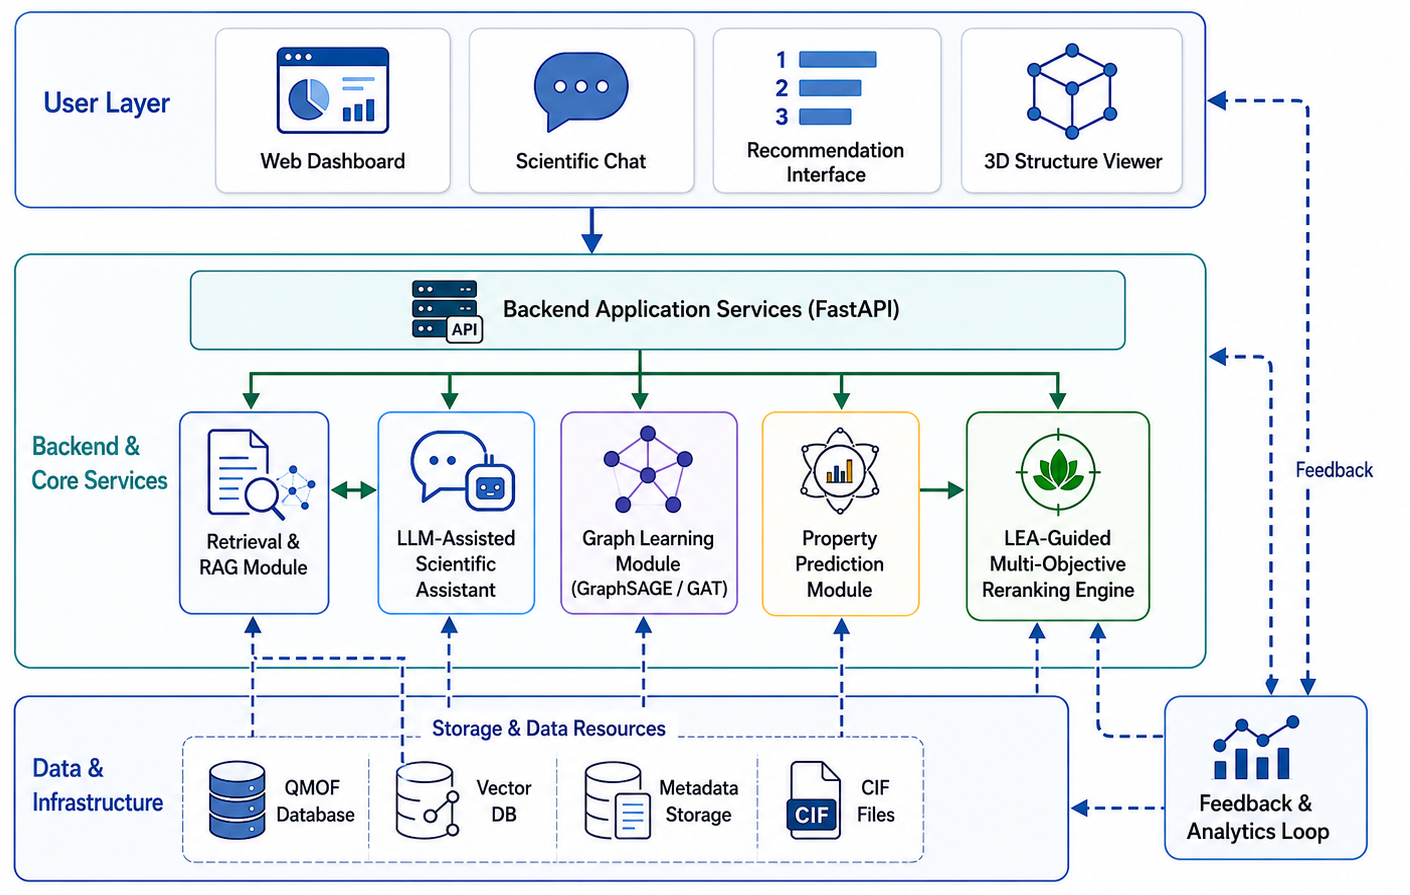
\includegraphics[width=\linewidth]{figures/fig1_architecture.png}
  \caption{Overview of the QMOF-Rec platform architecture. The system integrates user-facing interfaces, backend application services, retrieval-augmented generation, LLM-assisted scientific chat, formula-derived metadata-graph learning, property prediction, LEA-guided recommendation, data infrastructure, and feedback-driven analytics.}
  \label{fig:arch}
\end{figure}

\subsection{User Interaction and Frontend}

The user-facing layer supports a web dashboard, scientific chat assistant, recommendation interface, material detail cards, 3D structure/CIF viewer, and feedback interface. The recommendation interface exposes top-$K$ materials, objective contributions, and explanatory text. Material detail cards provide record-level metadata and, where available, structural files. The feedback interface records user judgments for later analytics, preference modeling, and possible continual-improvement workflows.

The frontend prototype was executed locally and inspected through browser-based screenshots (Figure~\ref{fig:frontend}). These views demonstrate the user-facing interaction layer of QMOF-Rec, including query input, the scientific chat interface, the recommendation interface, and analytics views. The screenshots are used only as implementation evidence and do not replace the offline ranking, graph, or ablation evaluations.

\begin{figure}[H]
  \centering
  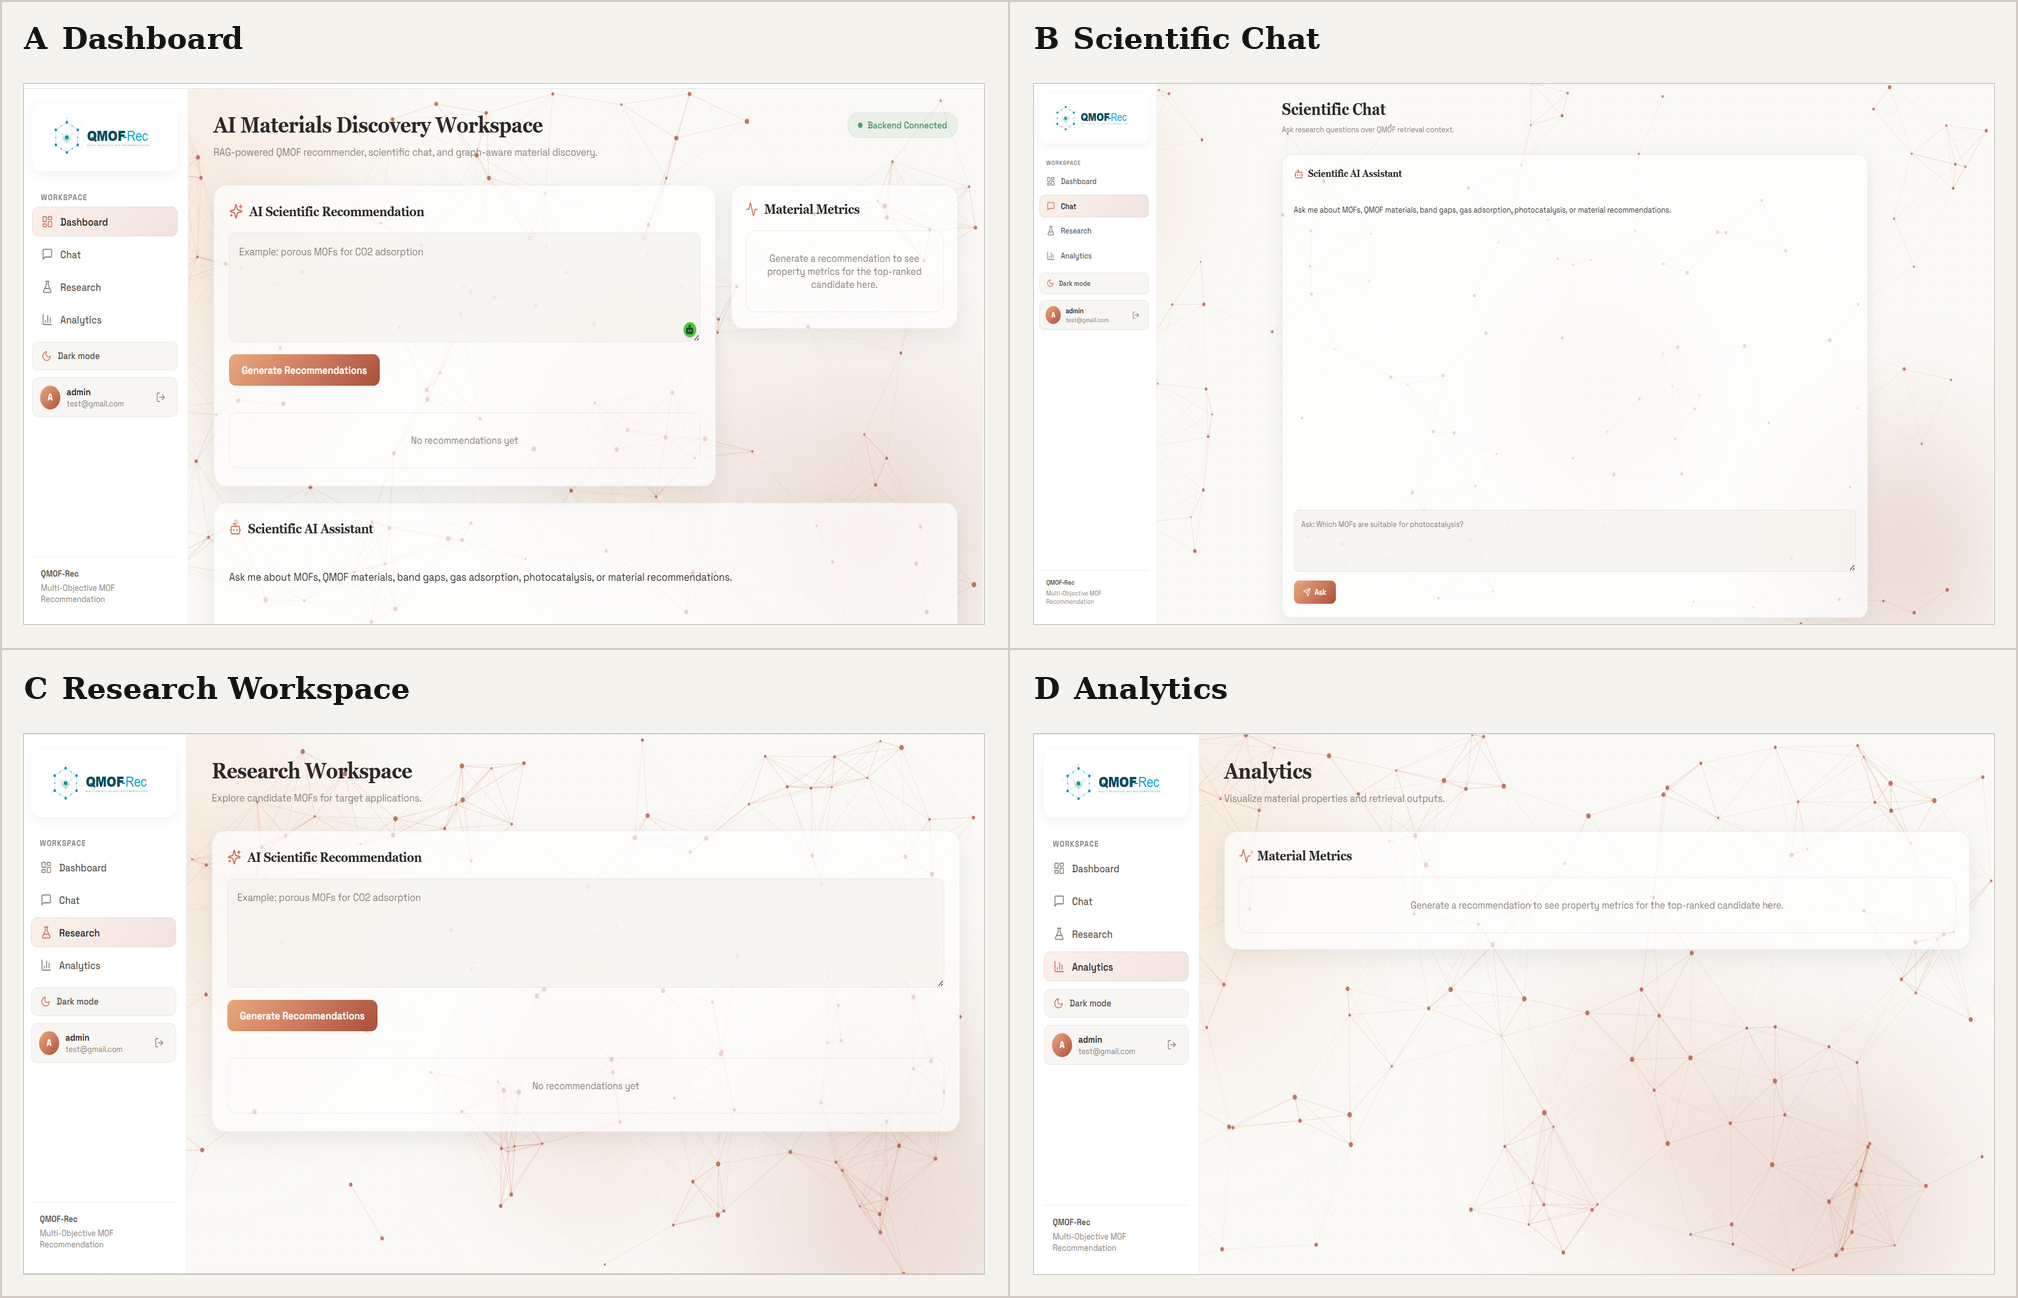
\includegraphics[width=0.85\linewidth]{figures/fig2_qmof_frontend.png}
  \caption{Compact QMOF-Rec application screenshot montage. Panel~A shows the recommendation workspace, Panel~B the scientific chat interface, Panel~C the research workspace, and Panel~D the analytics view. Screenshots demonstrate the implemented interface and are not part of the offline ranking validation.}
  \label{fig:frontend}
\end{figure}

\subsection{Backend and Application Services}

The backend layer is designed around a FastAPI application service pattern. The current repository defines routed services for chat, recommendation, material prediction uploads, and structure access, while flat \texttt{/feedback} and \texttt{/analytics} endpoints are platform-design targets rather than validated routes in the present rerun. Application services include an API gateway, recommendation service, chat/scientific-assistant service, property prediction service, graph construction service, RAG service, feedback/analytics service, and background jobs for indexing, embedding, graph generation, CIF processing, and model inference. Pydantic data models support typed request and response contracts.

\subsection{Data, Storage, and Infrastructure}

The data layer integrates the QMOF database, metadata tables, CIF/structure files, literature and papers, domain knowledge, and optional external public materials datasets. Storage and infrastructure include a metadata database, a vector database such as FAISS or pgvector, PostgreSQL-style tabular storage, Redis-like cache/queue support, file storage, logs, reports, and experiment outputs. The current reproducible evaluation uses vector metadata records and saved report artifacts rather than a fully rebuilt descriptor database.

\subsection{AI and Representation Layer}

The recommendation layer combines candidate generation, item representation, scoring, reranking, and explanation. Embedding models and metadata retrieval generate a candidate pool. Property scores, formula-derived metadata features, semantic signals, and graph embeddings represent candidate items. WeightedSum, TOPSIS, ParetoCrowding, SemanticOnly, Random, and MMR provide ranking baselines, while LEA performs multi-objective list-level reranking. A local graph-learning rerun constructs a formula-derived $k$-nearest-neighbor QMOF graph and evaluates GraphSAGE/GAT property-prediction and graph-aware recommendation variants; these results should be interpreted as metadata-graph baselines rather than CIF-derived atomic-graph benchmarks.

\subsection{Scientific Assistant and Feedback Layer}

The scientific assistant layer supports RAG retrieval, prompt construction, LLM orchestration, evidence-based explanations, recommendation rationales, confidence notes, and reference-supported answer generation. It generates text from retrieved evidence, candidate records, and QMOF metadata, while authoritative material-property values remain those stored in the underlying records. The feedback loop records user feedback, logging, analytics, and future model-improvement signals.

%% ════════════════════════════════════════════════════════════════════════════
\section{End-to-End Recommendation Scenario}
\label{sec:scenario}

This section illustrates how QMOF-Rec operates as a scientific recommender system from user request to final recommendation. Consider a materials scientist who enters the query: ``Recommend promising MOFs for CO$_2$ adsorption with low density and good stability.'' QMOF-Rec treats this input as a recommendation context rather than only as a text-search string. The system identifies semantic relevance to CO$_2$ adsorption, density, stability proxy, diversity, and optional graph-aware similarity as relevant objectives. Because void fraction is unavailable in the current metadata, porosity is not used as an active numerical objective.

The first stage is candidate generation. QMOF-Rec retrieves an initial candidate pool $C_q$ from the QMOF metadata/vector store. This stage is analogous to candidate generation in a two-stage recommender-system pipeline: it narrows the full QMOF item catalog to a smaller set of query-relevant materials. In the current reproducible evaluation, this pool contains 100 candidate QMOF records for each query scenario.

Each retrieved material is then represented as an item feature vector. Available descriptors and scores, including formula-derived signals, density, band gap where available, semantic metadata score, stability proxy, and metadata-derived objective scores, are normalized before ranking. Missing descriptors are handled explicitly. In particular, void fraction is absent in the current metadata, so the system avoids strong adsorption or porosity claims and communicates that limitation in the recommendation rationale.

If graph embeddings are available, QMOF-Rec can add a graph-aware signal from GraphSAGE/GAT models trained on the formula-derived metadata graph. This signal is useful as a local graph-neighborhood baseline, but it should not be interpreted as a CIF-derived atomistic graph result or as a physically validated structure-aware adsorption model.

The retrieved pool can be ranked by multiple baselines. WeightedSum provides the strongest relevance-oriented scoring baseline. TOPSIS ranks candidates by distance to ideal and anti-ideal solutions. ParetoCrowding emphasizes trade-offs and diversity. MMR provides a diversity-aware reranking reference. SemanticOnly and Random provide retrieval-only and chance-level controls. LEA is the active multi-objective reranker. In recommender-system terms, LEA acts as a multi-objective reranker whose diversity effect depends on the resolution and geometry of the selected material representation.

Table~\ref{tab:workflow} summarizes the complete workflow. The final output is a ranked top-$K$ list in which each recommendation can include the QMOF identifier, formula, available property values, method score, a short rationale, and a warning when relevant descriptors are missing. The candidate-conditioned explanation layer is evaluated for answer quality, groundedness, metadata consistency, unsupported-claim flags, limitation awareness, and explanation quality in Section~\ref{sec:rag_eval}; it is not evaluated as improving ranking quality. After inspecting candidate records or 3D/CIF structures where available, the user can mark materials as useful, uncertain, or irrelevant. Such feedback is stored for future expert review and possible preference-aware recommendation.

\begin{table}[H]
\centering
\caption{Example end-to-end QMOF-Rec recommendation scenario.}
\label{tab:workflow}
\small
\begin{tabular}{L{2.2cm} L{3.4cm} L{2.8cm} L{4.3cm}}
\toprule
\textbf{Step} & \textbf{System Action} & \textbf{RS Role} & \textbf{QMOF-Rec Output}\\
\midrule
User query & Interpret ``CO$_2$ adsorption with low density and good stability'' & Query/context capture & Weights for relevance, density, stability, diversity, and graph signal; porosity excluded when void fraction is unavailable\\
Candidate generation & Retrieve 100 query-relevant QMOF records & First-stage candidate generation & Candidate pool $C_q$\\
Objective scoring & Normalize available descriptors and metadata scores & Item representation and scoring & Objective matrix $X_q$ with missing-descriptor flags\\
Graph signal & Use formula-derived GraphSAGE/GAT embeddings when available & Hybrid signal & Metadata-graph similarity baseline\\
Baseline ranking & Apply deterministic and diversity-aware policies & Baseline top-$K$ ranking & Comparable ranked lists for offline evaluation\\
LEA reranking & Optimize relevance, balance, and diversity & List-level reranking & LEA-guided top-$K$ portfolio\\
Top-$K$ output & Return ranked QMOF candidates & User-facing recommendation & IDs, formulas, values, scores, and warnings\\
Explanation & Generate evidence-aware rationale & Explainable recommendation & Trade-off and uncertainty notes\\
Feedback & Record expert judgments & Future preference learning & Logs for review and later preference modeling\\
\bottomrule
\end{tabular}
\end{table}

Table~\ref{tab:co2_example} reports the final diversity-aware, mask-aware LEA top-5 recommendation output for the CO$_2$ adsorption scenario from the rerun artifact directory \path{artifacts/final_diversity_aware_masked_protocol/rankings}. The values should be interpreted under the metadata limitations above: density and band-gap values are available for these records, but void fraction is unavailable. Candidate ties in active utility scores are broken by the LEA fitness, which includes the selected diversity representation and deterministic candidate identifiers.

\begin{table}[H]
\centering
\caption{Example top-$K$ recommendations for the CO$_2$ adsorption scenario from the final diversity-aware, mask-aware rerun. Void-fraction values are unavailable in the current metadata. Scores are LEA optimization utilities, not probabilities.}
\label{tab:co2_example}
\small
\begin{tabular}{C{0.9cm} L{2.5cm} L{3.9cm} C{1.5cm} C{1.7cm} C{1.9cm}}
\toprule
\shortstack{\textbf{Rank}} & \textbf{QMOF ID} & \textbf{Formula} & \textbf{Density} & \shortstack{\textbf{Band}\\\textbf{gap}} & \shortstack{\textbf{LEA}\\\textbf{score}}\\
\midrule
1 & qmof-82fb334 & Co$_2$C$_{22}$H$_{16}$N$_4$O$_{10}$ & 1.773 & 2.754 & 0.847108\\
2 & qmof-ba8d316 & Co$_2$C$_{32}$H$_{24}$O$_{12}$ & 1.746 & 1.250 & 0.803574\\
3 & qmof-54f7ee7 & Co$_2$K$_2$C$_{48}$H$_{44}$N$_4$O$_6$ & 1.497 & 1.505 & 0.803149\\
4 & qmof-ec84fcf & Co$_2$C$_{20}$H$_{16}$N$_{28}$ & 1.767 & 2.596 & 0.801944\\
5 & qmof-330a403 & Co$_2$C$_{58}$F$_{12}$H$_{32}$N$_8$O$_8$S$_2$ & 1.415 & 2.471 & 0.801803\\
\bottomrule
\end{tabular}
\end{table}

The CO$_2$ scenario ranks candidates by balancing query relevance, density, band-gap-derived suitability, and stability proxy values under the available metadata. The missing void-fraction descriptor means these entries should be treated as recommendation candidates for expert follow-up rather than validated CO$_2$ uptake materials.

%% ════════════════════════════════════════════════════════════════════════════
\section{Problem Formulation}
\label{sec:formulation}

Let $\mathcal{M} = \{m_1, \ldots, m_{|\mathcal{M}|}\}$ denote the item catalog of QMOF material records and let $q$ denote a scientific query. In recommender-system terms, $q$ is the query context, $m_i$ is an item, and the goal is to return a ranked top-$K$ recommendation list. The initial candidate-generation stage returns a query-dependent candidate pool
\begin{equation}
  C_q = \{m_1, \ldots, m_n\} \subset \mathcal{M}.
  \label{eq:cq}
\end{equation}
Each candidate item $m_i$ is represented by a normalized active objective vector $\mathbf{x}_i \in [0,1]^d$ and an availability mask $\mathbf{a}_i \in \{0,1\}^d$. The mask entry $a_{ij}=1$ only when objective $j$ is observed or defensibly derived for material $m_i$; unsupported or missing descriptors have $a_{ij}=0$ and are excluded from active numerical scoring. This distinction prevents missing descriptors from being interpreted as physical zero values.
The query-specific weight vector is
\begin{equation}
  \mathbf{w}_q = (w_{q1}, \ldots, w_{qd}),\quad w_{qj} \geq 0,\quad \sum_{j=1}^{d} w_{qj} = 1.
\end{equation}
The objective matrix for the candidate pool is
\begin{equation}
  X_q = \begin{pmatrix} x_{11} & \cdots & x_{1d} \\ \vdots & \ddots & \vdots \\ x_{n1} & \cdots & x_{nd} \end{pmatrix},\quad x_{ij}\in[0,1].
\end{equation}
The corresponding availability matrix is
\begin{equation}
  A_q = \begin{pmatrix} a_{11} & \cdots & a_{1d} \\ \vdots & \ddots & \vdots \\ a_{n1} & \cdots & a_{nd} \end{pmatrix},\quad a_{ij}\in\{0,1\}.
\end{equation}
The recommender outputs a top-$K$ list $S_K \subset C_q$. Let $f(q, m_i, S)$ be the context-aware ranking or reranking utility of item $m_i$ for query $q$, optionally conditioned on the partial recommendation list $S$. The top-$K$ recommendation list is
\begin{equation}
  S_K(q) = \underset{m_i \in C_q}{\operatorname{TopK}}\; f(q, m_i, S).
\end{equation}
For deterministic pointwise rankers, $S$ is ignored. For list-aware reranking, $S$ captures the candidates already selected and enables diversity-aware portfolio construction. The masked weighted relevance score is
\begin{equation}
  R(m_i, q) =
  \frac{\sum_{j=1}^{d} a_{ij}w_{qj}x_{ij}}
       {\sum_{j=1}^{d} a_{ij}w_{qj}+\epsilon}.
  \label{eq:relevance}
\end{equation}
For a target property $p_i$ and query-specific target $\tau$, a normalized target score can be defined as
\begin{equation}
  s_{\mathrm{target}}(p_i;\tau) = \max\!\left(0, 1 - \frac{|p_i - \tau|}{r + \epsilon}\right),
\end{equation}
where $r$ is a normalization range and $\epsilon$ avoids division by zero. The masked balance score is
\begin{equation}
  B(m_i) =
  \begin{cases}
  1-\sqrt{\dfrac{1}{\sum_j a_{ij}}\displaystyle\sum_{j:a_{ij}=1}\left(x_{ij}-\bar{x}_{i,\mathrm{obs}}\right)^2}, & \sum_j a_{ij} > 0,\\[8pt]
  0, & \sum_j a_{ij}=0.
  \end{cases}
\end{equation}
where $\bar{x}_{i,\mathrm{obs}}$ is the mean of the observed active objectives for candidate $m_i$; the implementation clips this score to $[0,1]$. For two candidates, the joint availability indicator is $a_{i\ell,j}=a_{ij}a_{\ell j}$. Masked cosine similarity is computed only over jointly observed dimensions and is used for auxiliary material-similarity scoring:
\begin{equation}
  \cos_{\mathrm{mask}}(\mathbf{x}_i,\mathbf{x}_\ell)=
  \frac{\sum_{j:a_{i\ell,j}=1}x_{ij}x_{\ell j}}
       {\sqrt{\sum_{j:a_{i\ell,j}=1}x_{ij}^2}\sqrt{\sum_{j:a_{i\ell,j}=1}x_{\ell j}^2}+\epsilon}.
\end{equation}
If no jointly observed dimension exists, or if the denominator is zero, the implemented fallback returns zero similarity. With one jointly observed dimension, the same one-dimensional cosine expression is used. The final implementation separates candidate remapping in active objective space from list diversity in hybrid material space.

The objective-space distance used for LEA candidate remapping is
\begin{equation}
  d_{\mathrm{obj}}(\mathbf{x}_i,\mathbf{x}_\ell)=
  \begin{cases}
  \sqrt{\dfrac{\sum_{j:a_{i\ell,j}=1}(x_{ij}-x_{\ell j})^2}{\sum_j a_{i\ell,j}}}, & \sum_j a_{i\ell,j}>0,\\[8pt]
  0, & \sum_j a_{i\ell,j}=0.
  \end{cases}
\end{equation}
The final diversity representation $\mathbf{h}_i$ is distinct from $\mathbf{x}_i$. It concatenates a two-dimensional physical vector $\mathbf{p}_i$ containing full-catalog min--max-normalized density and band gap, an eight-dimensional formula vector $\mathbf{f}_i$ containing C, H, N, O, metal, and heteroatom fractions plus scaled atom and element counts, and a two-dimensional graph-proxy vector $\mathbf{g}_i$ containing formula-derived GraphSAGE and GAT proxy scores:
\begin{equation}
  \mathbf{h}_i =
  \left[
  \sqrt{\frac{0.55}{2}}\mathbf{p}_i\;\middle\|\;
  \sqrt{\frac{0.30}{8}}\mathbf{f}_i\;\middle\|\;
  \sqrt{\frac{0.15}{2}}\mathbf{g}_i
  \right].
\end{equation}
Density and band gap are normalized globally over the 20{,}372-record catalog rather than within each candidate pool. Missing band gap is masked and excluded from pairwise distance; density is available for all records; formula and graph-proxy features are available for all formula-bearing records; void fraction is excluded. Graph features are engineered formula-derived proxy scores, not trained CIF-derived embeddings. Full precision is used in calculations, and rounding is applied only for display.

The hybrid material distance is the same masked root-mean-square form applied to $\mathbf{h}_i$:
\begin{equation}
  d_{\mathrm{hybrid}}(\mathbf{h}_i,\mathbf{h}_\ell)=
  \begin{cases}
  \sqrt{\dfrac{\sum_{j:b_{i\ell,j}=1}(h_{ij}-h_{\ell j})^2}{\sum_j b_{i\ell,j}}}, & \sum_j b_{i\ell,j}>0,\\[8pt]
  0, & \sum_j b_{i\ell,j}=0,
  \end{cases}
\end{equation}
where $b_{i\ell,j}$ is the joint availability indicator for the hybrid feature dimension. The diversity score relative to a partial list $S$ is
\begin{equation}
  D_{\mathrm{hybrid}}(m_i,S)=
  \begin{cases}
  0, & |S|=0,\\[4pt]
  \dfrac{1}{|S|}\displaystyle\sum_{m_j\in S}d_{\mathrm{hybrid}}(\mathbf{h}_i,\mathbf{h}_j), & |S|>0.
  \end{cases}
\end{equation}
QMOF-Rec defines the list-aware multi-objective utility as
\begin{equation}
  f(q,m_i,S) = \alpha R(m_i,q) + \beta B(m_i) + \gamma D_{\mathrm{hybrid}}(m_i,S) + \eta G(m_i,q) + \delta N(m_i),
  \label{eq:utility}
\end{equation}
where $R$ is query relevance, $B$ is objective balance, $D_{\mathrm{hybrid}}$ is diversity relative to the partial list, $G$ is optional graph-aware similarity, and $N$ is optional novelty. The current repository implementation uses $\alpha=1.0$, $\beta=0.10$, $\gamma=0.10$, $\eta=0$ for non-graph reranking, and a redundancy penalty of $0.05\exp[-D_{\mathrm{hybrid}}(m_i,S)]$ inside LEA fitness. The hybrid representation was selected before the final method comparison using criteria of feature availability, full-precision continuity, interpretability, reproducibility, missing-value compatibility, and absence of target leakage rather than by optimizing LEA's reported performance.

%% ════════════════════════════════════════════════════════════════════════════
\section{Retrieval-Augmented Scientific Assistance}
\label{sec:rag_form}

Let $\mathcal{D} = \{d_1, \ldots, d_M\}$ be the document and metadata corpus. Each document chunk is embedded as $\mathbf{e}_i = f_\theta(d_i)$, and the query is embedded as $\mathbf{e}_q = f_\theta(q)$. The implemented FAISS retrieval index uses squared L2 distance, so the retrieved evidence set is
\begin{equation}
  \mathcal{R}_K(q) = \underset{d_i\in\mathcal{D}}{\operatorname{TopK}}\;[-\|\mathbf{e}_q-\mathbf{e}_i\|_2^2],
\end{equation}
where smaller FAISS L2 distance corresponds to higher retrieval rank. This equation describes the live retrieval store; the offline ranking tables use the deterministic semantic proxy described above.
The augmented LLM input is
\begin{equation}
  A(q) = \operatorname{Template}(q, \mathcal{R}_K(q), C_q, X_q, \mathbf{w}_q),
\end{equation}
and the generated scientific response is $y = \operatorname{LLM}_\phi(A(q))$.

The scientific-assistant component generates explanations from retrieved evidence, candidate records, and QMOF metadata. Authoritative material-property values are taken from the underlying records rather than generated text. The candidate-conditioned explanation layer is evaluated in Section~\ref{sec:rag_eval} for answer quality, groundedness, metadata consistency, unsupported-claim flags, limitation awareness, and explanation quality under automated checks. It is not evaluated as improving ranking quality. Expert human evaluation, citation-fidelity assessment, and user-usefulness studies remain future work.

%% ════════════════════════════════════════════════════════════════════════════
\section{Graph-Aware QMOF Representation Learning}
\label{sec:graph}

The QMOF materials graph is defined as $\mathcal{G} = (\mathcal{V}, \mathcal{E})$, where each node $v_i \in \mathcal{V}$ represents a QMOF material and each edge $(v_i, v_j) \in \mathcal{E}$ represents a relationship between two materials. Edges can be constructed from structural similarity, descriptor similarity, text/embedding similarity, shared metal chemistry, shared linker chemistry, topology similarity, guest-accessibility similarity, or $k$-nearest-neighbor relations in descriptor space.

The initial node representation can be written as
\begin{equation}
  \mathbf{h}_i^{(0)} = [\mathbf{x}_i,\; \mathbf{p}_i,\; \mathbf{s}_i],
\end{equation}
where $\mathbf{x}_i$ is the normalized recommendation objective vector, $\mathbf{p}_i$ contains physico-chemical descriptors, and $\mathbf{s}_i$ contains semantic or structural embeddings.

GraphSAGE supports inductive representation learning for unseen or newly added QMOFs by aggregating neighbor representations:
\begin{equation}
  \mathbf{h}_v^{(k)} = \sigma\!\left(W^{(k)}\cdot\left[\mathbf{h}_v^{(k-1)}\;\Big\|\;\operatorname{AGG}^{(k)}\!\left\{\mathbf{h}_u^{(k-1)}:u\in\mathcal{N}(v)\right\}\right]\right).
\end{equation}
Here, $\mathcal{N}(v)$ is the neighborhood of node $v$, AGG may be a mean, max, or LSTM-style aggregation function, and $\|$ denotes concatenation.

GAT learns attention weights over neighboring materials. The attention coefficient is
\begin{equation}
  \alpha_{vu} = \frac{\exp\!\left(\operatorname{LeakyReLU}\!\left(\mathbf{a}^\top[W\mathbf{h}_v\|W\mathbf{h}_u]\right)\right)}{\sum_{r\in\mathcal{N}(v)}\exp\!\left(\operatorname{LeakyReLU}\!\left(\mathbf{a}^\top[W\mathbf{h}_v\|W\mathbf{h}_r]\right)\right)}.
\end{equation}
Here, $W$ is a trainable linear transformation, $\mathbf{a}$ is a trainable attention vector, and the denominator normalizes attention over neighbors $r \in \mathcal{N}(v)$. The GAT update is
\begin{equation}
  \mathbf{h}_v' = \sigma\!\left(\sum_{u\in\mathcal{N}(v)}\alpha_{vu}\,W\mathbf{h}_u\right).
\end{equation}
GraphSAGE can support inductive updates when new QMOFs are added to the platform, while GAT can expose learned neighbor importance. In the current manuscript, the reproduced graph-learning results use a formula-derived metadata graph. They are not presented as CIF-derived, atomistic, or full structure-aware GNN results.

%% ════════════════════════════════════════════════════════════════════════════
\section{Integration of Graph Embeddings into Recommendation}
\label{sec:graph_int}

Let the graph embedding of a material be $\mathbf{g}_i = \operatorname{GNN}(\mathcal{G}, \mathbf{h}_i^{(0)})$. A graph similarity score can be defined as $s_{\mathrm{graph}}(m_i, q) = \cos(\mathbf{g}_i, \mathbf{g}_q)$, where $\mathbf{g}_q$ may be obtained by aggregating graph embeddings of initially retrieved candidates or by projecting the query embedding into graph-embedding space.

The graph-aware objective vector becomes
\begin{equation}
  \tilde{\mathbf{x}}_i = [s_{\mathrm{sem}}(m_i,q),\; s_{\mathrm{bandgap}}(m_i),\; s_{\mathrm{density}}(m_i),\; s_{\mathrm{stability}}(m_i),\; s_{\mathrm{graph}}(m_i,q)].
\end{equation}
Descriptor availability is tracked by a binary mask $\mathbf{a}_i \in \{0,1\}^{d+1}$, where $a_{ij}=1$ only when objective $j$ is observed or defensibly derived for material $m_i$. The updated weighted relevance is
\begin{equation}
  R(m_i,q) =
  \frac{\sum_{j=1}^{d+1} a_{ij}\tilde{w}_{qj}\tilde{x}_{ij}}
       {\sum_{j=1}^{d+1} a_{ij}\tilde{w}_{qj}+\epsilon}.
\end{equation}
Graph-aware relevance and candidate remapping use the active objective vector with the graph-similarity term appended when that variant is enabled. Final list diversity remains computed with the hybrid material distance defined above, not with the graph-aware objective vector alone. This extension makes the recommender graph-aware while preserving the distinction between missing descriptors and genuine zero values. Structurally meaningful candidates can be promoted when metadata are incomplete or when semantic metadata do not fully describe material similarity. Graph embeddings should be treated as an additional scientific signal, not as a replacement for property validation, adsorption simulation, synthesis feasibility analysis, or expert review.

%% ════════════════════════════════════════════════════════════════════════════
\section{LEA-Guided Multi-Objective Reranking}
\label{sec:lea}

The original LEA algorithm is a lotus-nature-inspired metaheuristic introduced for engineering design optimization \cite{dalirinia2024}. The LEA-rec adaptation implemented here uses the same broad intuition of adaptive exploration and self-cleaning but operates as a post-retrieval reranker over normalized recommendation objectives. Individuals move in continuous normalized objective space, but final recommendations must always map back to valid QMOF records.

The candidate-validity mapping uses the active objective-space masked distance, whereas final reported list diversity uses the hybrid material distance:
\begin{equation}
  \pi(\mathbf{z}) = \arg\min_{m_i \in C_q}d_{\mathrm{obj}}(\mathbf{z},\mathbf{x}_i),
\end{equation}
where the candidate mask $\mathbf{a}_i$ determines which active objectives participate in the remapping distance. The implementation uses iteration-dependent Gaussian exploration and exploitation toward the current best solution:
\begin{equation}
  \mathbf{z}_i^{t+1} =
  \operatorname{clip}_{[0,1]}\!\left(\mathbf{z}_i^t
  + \boldsymbol{\epsilon}_t
  + \frac{t}{T}(\mathbf{g}^t-\mathbf{z}_i^t)\right),
\end{equation}
where $t$ is the current iteration, $T$ is the maximum iteration count, $\mathbf{g}^t$ is the current best solution, and $\boldsymbol{\epsilon}_t \sim \mathcal{N}(0,(0.20(1-t/T))^2I)$. The clipping operation keeps solutions inside the normalized objective domain.

The self-cleaning replacement step is applied every $\tau = 10$ iterations in the implemented code. The weakest fraction of the population is replaced by random normalized vectors:
\begin{equation}
  P^{t+1}_{\mathrm{weak}} \leftarrow \{u_1,\ldots,u_{\lceil\rho N\rceil}\},\quad u_j \sim \mathcal{U}(0,1)^d,
\end{equation}
with $\rho = 0.15$ in the current implementation. This replacement increases exploration and helps avoid portfolios that collapse into a narrow region of the objective space.

%% ════════════════════════════════════════════════════════════════════════════
\section{Workflow Summary}
\label{sec:algorithms}

The computational workflow has three stages. First, QMOF-Rec retrieves a query-dependent candidate pool from metadata and text representations. Second, it converts candidate records into active objective vectors with descriptor-availability masks, excluding unsupported descriptors from numerical relevance and balance while using a richer masked material representation for diversity. Third, LEA-guided reranking constructs a top-$K$ portfolio and the candidate-conditioned explanation layer generates an evidence-grounded explanation. Full pseudocode for retrieval/objective scoring, LEA reranking, and graph-aware explanation assistance is provided in the supplementary material.

%% ════════════════════════════════════════════════════════════════════════════
\section{Experimental Setup}
\label{sec:setup}

The current evaluation uses 20{,}372 QMOF vector metadata records. Density is available for all materials. Band gap is available for 10{,}810 materials, corresponding to approximately 53.1\% coverage. Void fraction is absent in the current metadata. Figure~\ref{fig:coverage} summarizes this descriptor coverage.

\begin{figure}[H]
  \centering
  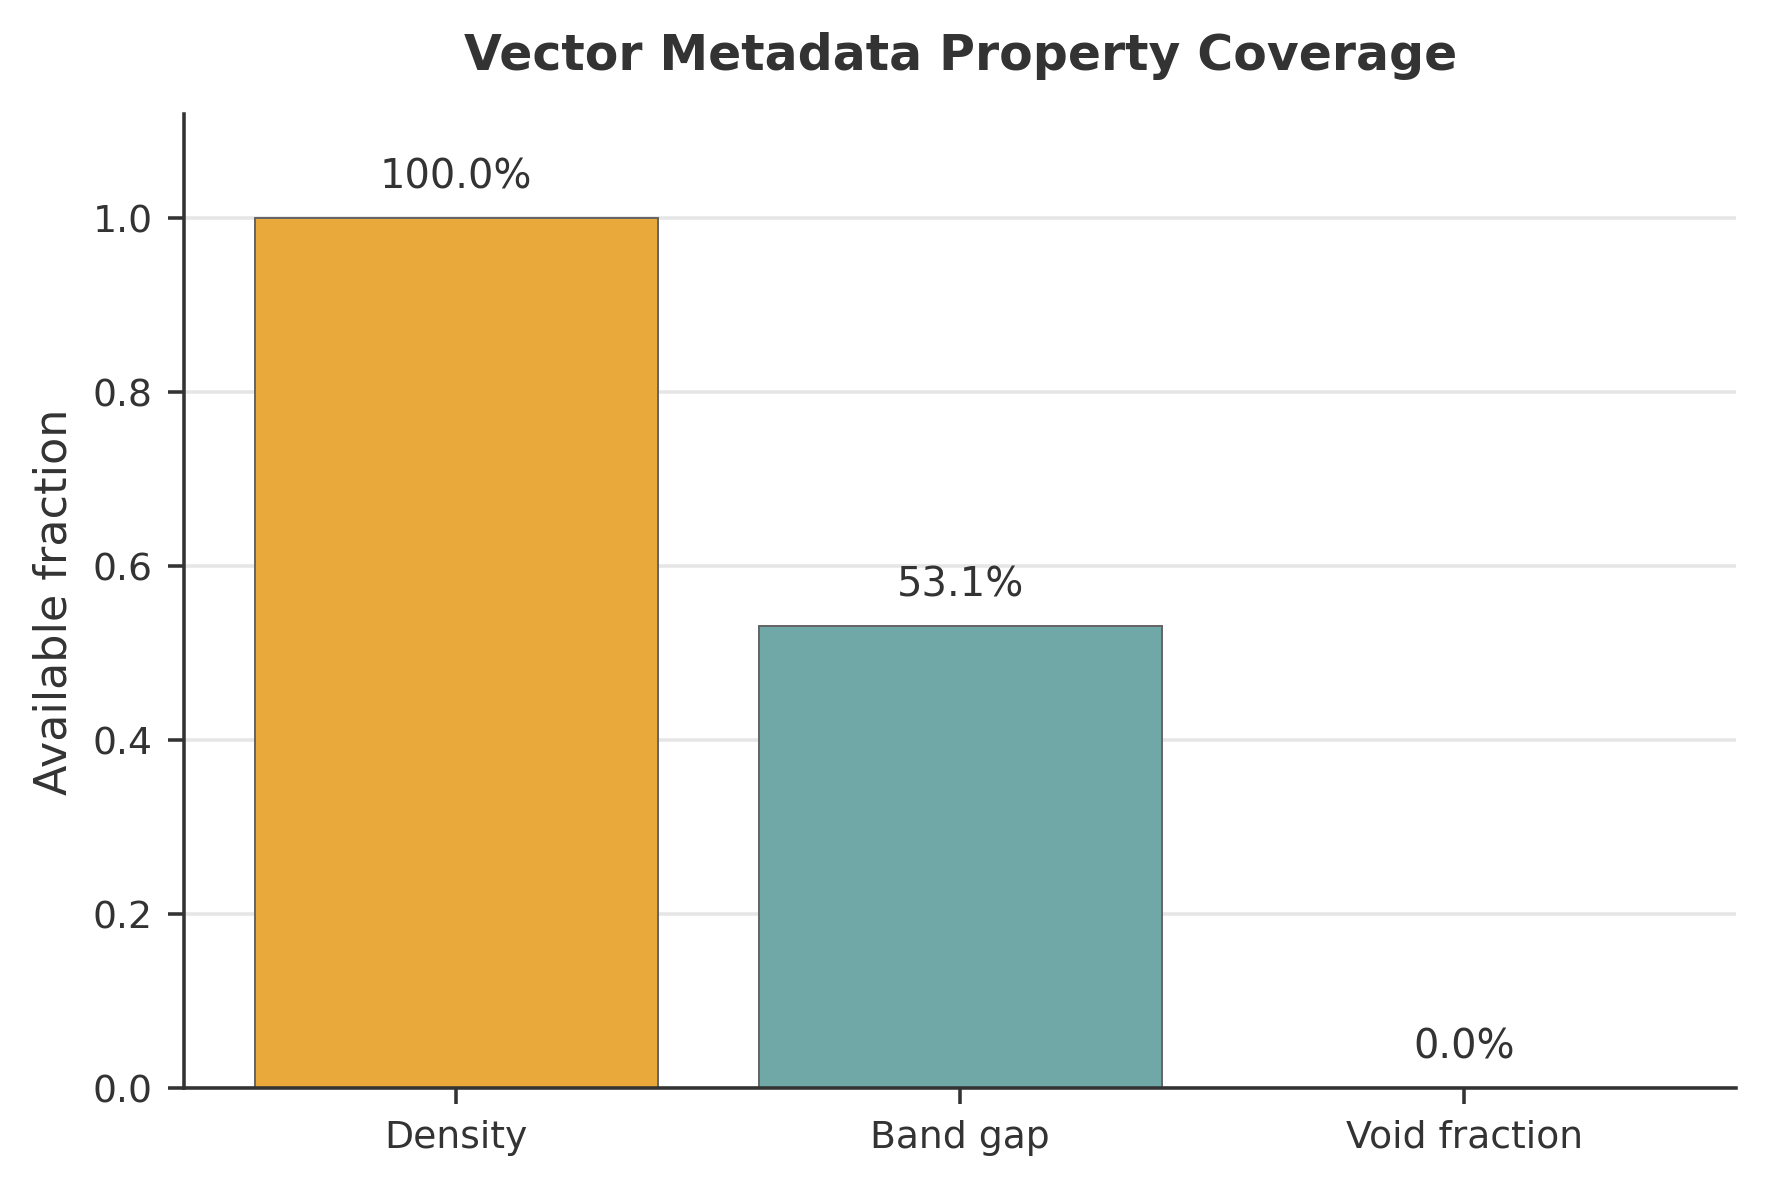
\includegraphics[width=0.6\linewidth]{figures/figure_2_data_coverage.png}
  \caption{Coverage of metadata fields used in the current reproducible QMOF-Rec evaluation. Density is available for all records, band gap is partially available, and void fraction is absent.}
  \label{fig:coverage}
\end{figure}

The missing void-fraction field materially affects interpretation. The current evaluation supports density-aware and partial band-gap-aware ranking. It does not support strong porosity-aware, adsorption-specific, or CO$_2$ uptake claims. CO$_2$ adsorption recommendations should be read as preliminary recommendation behavior under incomplete metadata, not as validated adsorption screening.

Five query scenarios are evaluated: CO$_2$ adsorption, photocatalysis, lightweight gas storage, balanced discovery, and wide-band-gap insulating frameworks. Each scenario retrieves a candidate pool of 100 materials and returns a top-$K$ list with $K=5$. The main ranking evaluation compares SemanticOnly, WeightedSum, TOPSIS, ParetoCrowding, Random, and LEA. A separate ablation and graph-aware evaluation reports MMR, LEA no diversity, LEA no self-clean, GraphSAGE-only, GAT-only, LEA+GraphSAGE, and LEA+GAT using the formula-derived metadata graph. The supplementary material reports retrieval missingness, query-stratified repeated-seed summaries, variance decomposition, available candidate-pool-size sensitivity results, the LEA-no-diversity metric identity check, and an observed physical-descriptor plot comparing all records with selected top-$K$ portfolios. Future baselines not implemented in the current repository include Non-dominated Sorting Genetic Algorithm II (NSGA-II), particle swarm optimization (PSO), genetic algorithm (GA), Bayesian optimization, learning-to-rank methods, and expert-labeled supervised metrics.

%% ════════════════════════════════════════════════════════════════════════════
\section{Recommendation Evaluation Metrics}
\label{sec:metrics}

\subsection{Offline Recommendation Protocol Without User Histories}

Because no historical user-click or rating log exists for QMOF materials, the evaluation follows an offline query-driven recommendation protocol. QMOF-Rec is a hybrid scientific recommender with a strong content-based focus: it does not rely on collaborative filtering because no large-scale user--MOF interaction log is available. The task is similar to session-based or context-aware recommendation, where the query supplies the current user intent and item content supplies the ranking evidence. User feedback is included architecturally for future online learning, but the present evaluation uses query-dependent objective weights rather than user ratings.

\subsection{Ranking, Diversity, and Coverage Metrics}

Mean relevance is computed as
\begin{equation}
  \mathrm{Rel}@K(S_K) = \frac{1}{K}\sum_{m_i \in S_K} R(m_i, q).
\end{equation}
If binary or graded expert labels become available, Precision@$K$ can be computed as $\mathrm{Precision}@K(S_K) = \frac{1}{K}\sum_{m_i\in S_K}\mathbf{1}[\mathrm{rel}(m_i,q)\geq\theta]$, where $\theta$ is a relevance threshold. In the current offline protocol, no expert-labeled relevant set is available, so Precision@$K$ is defined as a future supervised recommender-system metric. Discounted cumulative gain is
\begin{equation}
  \mathrm{DCG}@K = \sum_{r=1}^{K}\frac{2^{\mathrm{rel}_r}-1}{\log_2(r+1)},
\end{equation}
and normalized discounted cumulative gain is $\mathrm{NDCG}@K = \mathrm{DCG}@K / \mathrm{IDCG}@K$. The final rerun keeps relevance scoring on the mask-aware active utility vector, but computes intra-list diversity (ILD) over a full-precision hybrid material representation containing observed density, observed band gap, formula-derived descriptors, and formula-derived graph proxies:
\begin{equation}
  \mathrm{ILD}_{\mathrm{hybrid}}(S_K) = \frac{2}{K(K-1)}\sum_{i<j}d_{\mathrm{hybrid}}(\mathbf{h}_i,\mathbf{h}_j).
\end{equation}
The hybrid distance masks missing physical dimensions, excludes void fraction, and uses full precision before any manuscript rounding. This representation is used for final diversity, ParetoCrowding crowding distance, MMR redundancy, and LEA list-level diversity. Unique@$K$ is the fraction of unique items within a top-$K$ list and is distinct from catalog coverage.
Catalog coverage measures how much of the item space is recommended across a query set $\mathcal{Q}$:
\begin{equation}
  \mathrm{Coverage} = \frac{\left|\bigcup_{q\in\mathcal{Q}}S_K(q)\right|}{|\mathcal{M}|}.
\end{equation}
The ablation rerun also reports top-$K$ uniqueness coverage within each recommendation list. Runtime is reported as mean runtime in milliseconds. The reported hypervolume value is a hypervolume proxy rather than exact Pareto hypervolume, computed from the product-like multi-objective footprint used by the reproducible evaluation script and should be interpreted as a comparative proxy only.

All ranking results below were regenerated with the final diversity-aware, mask-aware implementation, the configuration in \path{configs/final_diversity_aware_masked_protocol.json}, and shared candidate pools for all ranking methods. Historical and prior final-masked protocol outputs are preserved only for comparison in the supplementary artifacts.

%% ════════════════════════════════════════════════════════════════════════════
\section{Recommendation Performance: Ranking Quality and Portfolio Diversity}
\label{sec:results}

Table~\ref{tab:ranking} reports the final diversity-aware, mask-aware aggregate top-$K$ recommendation results. WeightedSum, TOPSIS, MMR, and baseline LEA tie on the relevance-aligned metrics in this deterministic proxy evaluation. The diversity diagnosis showed that the prior zero-diversity result was caused by binned utility scores used for distance, not by identical raw density or band-gap values. Under the final hybrid material distance, baseline LEA shows a modest diversity difference relative to WeightedSum (0.0224 versus 0.0187), while MMR gives the highest diversity among relevance-preserving primary methods (0.0241) at higher runtime.

Figures~\ref{fig:comparison}--\ref{fig:radar} summarize the final diversity-aware evaluation from complementary perspectives. Figure~\ref{fig:comparison} separates relevance/NDCG from diversity, Figure~\ref{fig:runtime} reports runtime on a logarithmic axis, Figure~\ref{fig:convergence} shows representative seed-42 LEA convergence behavior across query scenarios, and Figure~\ref{fig:radar} compares aggregate method profiles after excluding unavailable porosity information.

\begin{table}[H]
\centering
\caption{Aggregate ranking results from the final diversity-aware, mask-aware QMOF-Rec rerun. Higher is better for Rel@5, Diversity, NDCG@5, and the hypervolume proxy; lower is better for runtime. Bold denotes the best value and underline denotes the second-best value; tied best values are bolded and tied second-best values are underlined equally. Hypervolume is reported as a proxy rather than exact Pareto hypervolume.}
\label{tab:ranking}
\small
\begin{tabular}{L{2.8cm} C{1.4cm} C{1.6cm} C{1.6cm} C{2.4cm} C{2.2cm}}
\toprule
\textbf{Method} & \textbf{Rel@5} & \shortstack{\textbf{Diversity}} & \shortstack{\textbf{NDCG}\\\textbf{@5}} & \shortstack{\textbf{Hyper-}\\\textbf{volume}} & \shortstack{\textbf{Runtime}\\\textbf{(ms)}}\\
\midrule
WeightedSum    & \textbf{0.8479} & 0.0187 & \textbf{1.0000} & 0.0121 & \underline{0.05}\\
LEA            & \textbf{0.8479} & 0.0224 & \textbf{1.0000} & \underline{0.0141} & 83.92\\
TOPSIS         & \textbf{0.8479} & 0.0187 & \textbf{1.0000} & 0.0121 & 1.02\\
ParetoCrowding & \underline{0.8447} & \textbf{0.0263} & \underline{0.9952} & 0.0125 & 215.59\\
MMR            & \textbf{0.8479} & \underline{0.0241} & \textbf{1.0000} & \textbf{0.0150} & 2114.36\\
Random         & 0.7695 & 0.0237 & 0.8809 & 0.0067 & \underline{0.05}\\
SemanticOnly   & 0.7600 & 0.0240 & 0.8678 & 0.0057 & \textbf{0.03}\\
\bottomrule
\end{tabular}
\end{table}

\begin{figure}[H]
  \centering
  
\includegraphics[width=\linewidth]{figures/figure_3_metric_comparison.png}
  \caption{Aggregate ranking metric comparison for SemanticOnly, WeightedSum, TOPSIS, ParetoCrowding, Random, MMR, and LEA. Rel@5/NDCG@5 and diversity are plotted in separate panels to avoid compressing the smaller diversity values.}
  \label{fig:comparison}
\end{figure}

\begin{figure}[H]
  \centering
  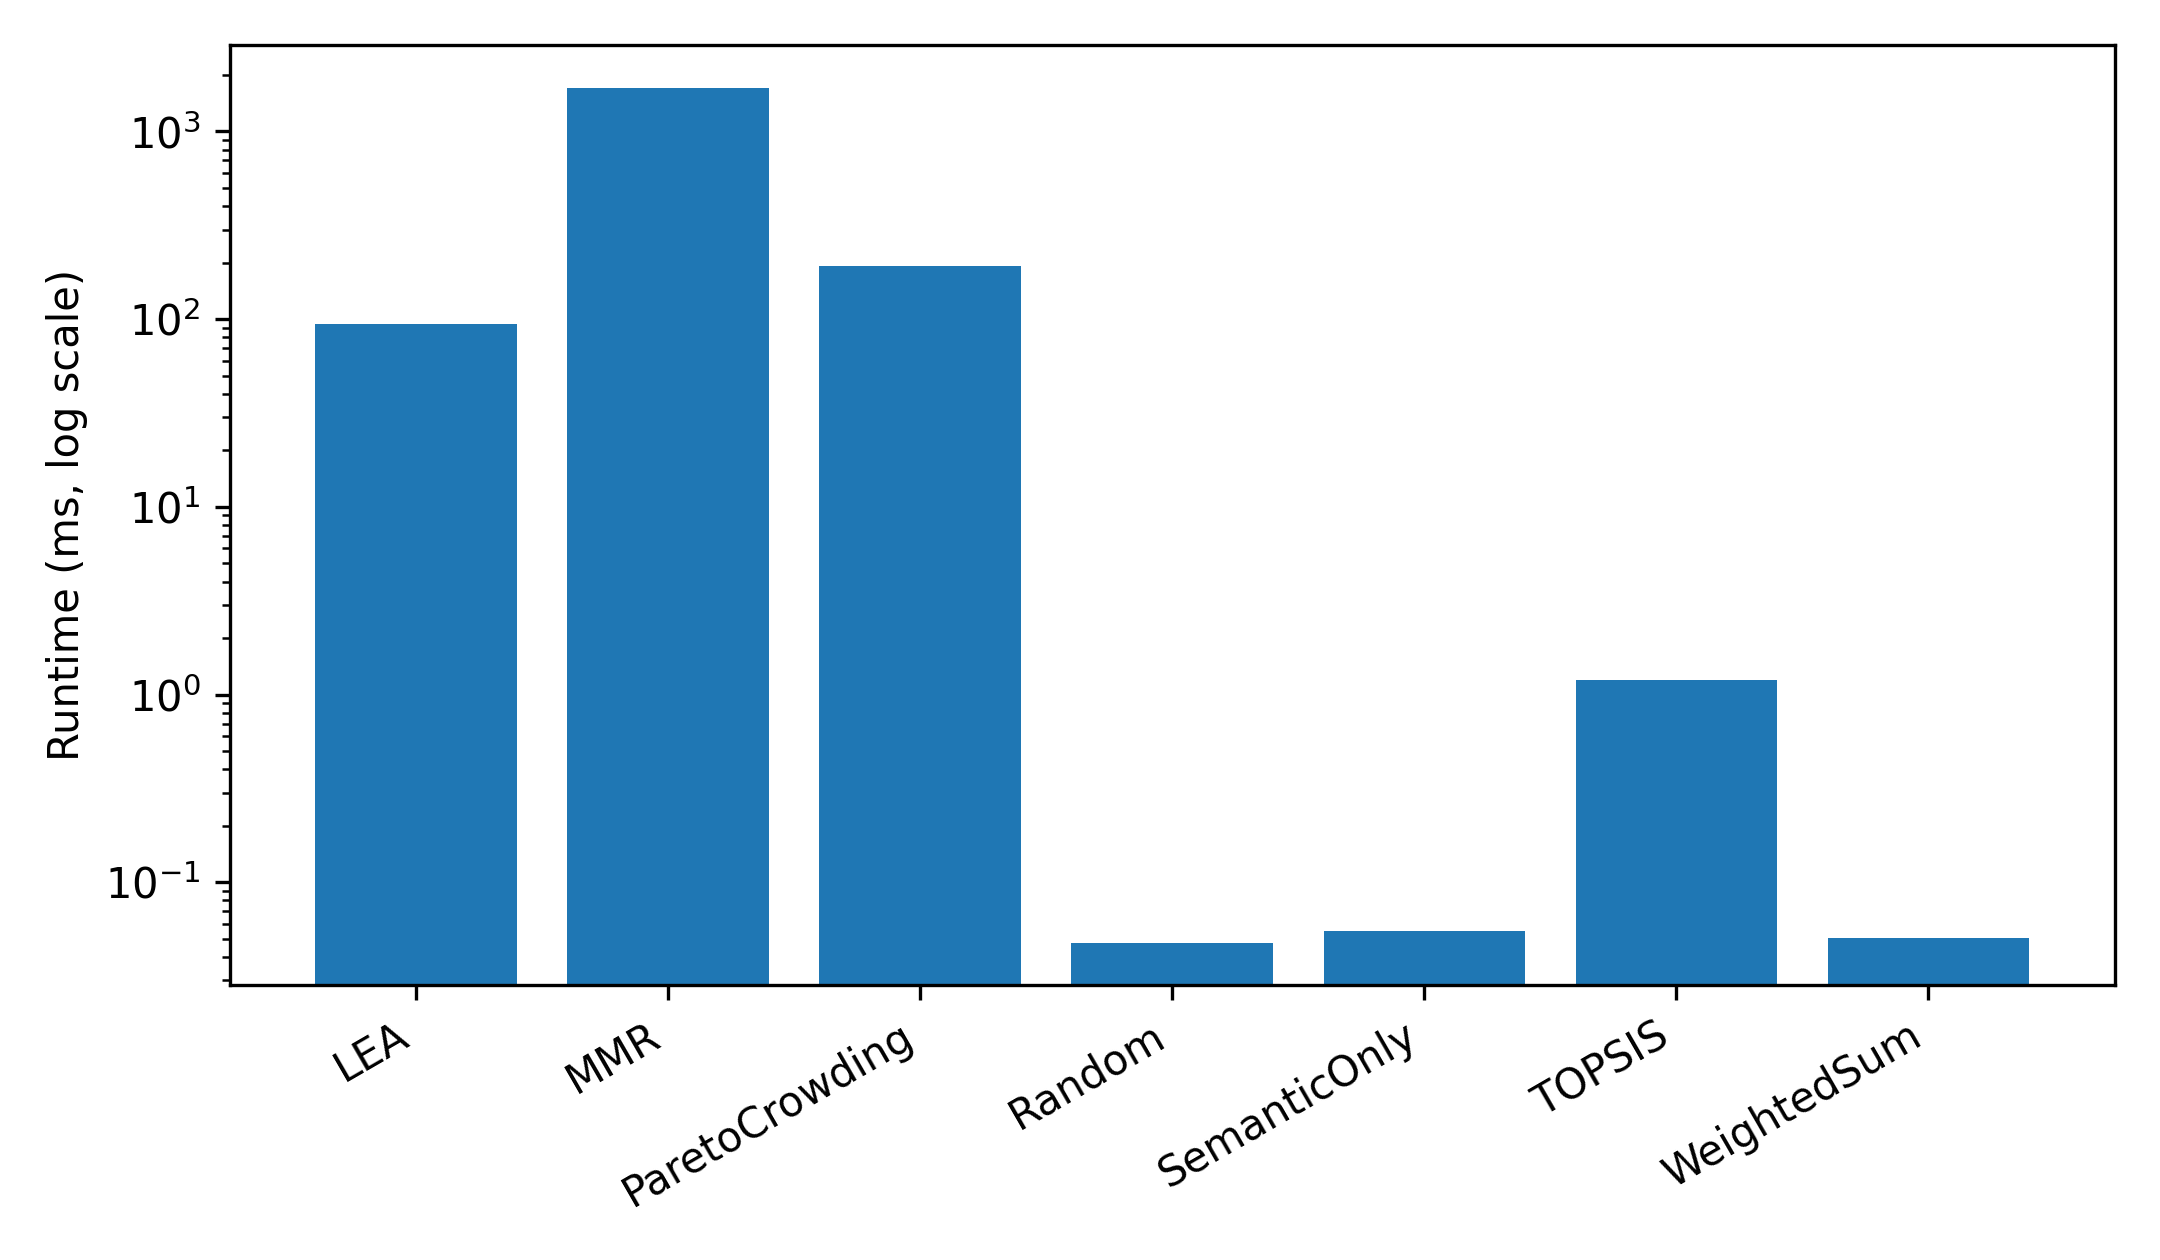
\includegraphics[width=0.72\linewidth]{figures/figure_4_runtime_log.png}
  \caption{Runtime comparison for SemanticOnly, WeightedSum, TOPSIS, ParetoCrowding, Random, MMR, and LEA. The y-axis uses a logarithmic scale; SemanticOnly, WeightedSum, and Random are below 0.1\,ms on average, TOPSIS is approximately 1.0\,ms, LEA is approximately 83.9\,ms, ParetoCrowding is approximately 215.6\,ms, and MMR is slowest at approximately 2114\,ms.}
  \label{fig:runtime}
\end{figure}

\begin{figure}[H]
  \centering
  
\includegraphics[width=0.72\linewidth]{figures/figure_5_lea_convergence.png}
  \caption{Representative LEA convergence traces for seed 42 across the evaluated query scenarios under the final hybrid material diversity representation.}
  \label{fig:convergence}
\end{figure}

\begin{figure}[H]
  \centering
  
\includegraphics[width=0.62\linewidth]{figures/figure_6_objective_radar.png}
  \caption{Aggregate method radar profiles comparing WeightedSum, MMR, LEA, and graph-aware LEA variants. Values are means over the evaluated query/seed runs. The axes report Rel@5, NDCG@5, list-level hybrid material diversity, normalized band-gap score, and normalized density score. Void fraction is unavailable for all 20{,}372 records and is excluded.}
  \label{fig:radar}
\end{figure}

The main empirical conclusion is conservative. The final rerun shows that representation choice matters: active utility-score diversity collapses because binned property scores hide continuous material differences, whereas hybrid material diversity recovers measurable list variation. Baseline LEA remains tied with WeightedSum on Rel@5 and NDCG@5 and gives a modest diversity gain under the selected representation. MMR remains the most diverse relevance-preserving primary method, but it is much slower. Graph-aware variants preserve the best relevance values, although the graph signal is formula-derived rather than CIF-derived.

\subsection{Example Recommendation Scenarios}

Table~\ref{tab:examples} reports the highest-ranked LEA recommendation for each evaluated query scenario from the final diversity-aware, mask-aware rerun. These examples illustrate the recommendation use case and should be read as offline recommendation outputs, not as experimentally validated discoveries.

For CO$_2$ adsorption, the recommender balances query relevance, density, and stability-oriented signals while excluding porosity from numerical ranking because void fraction is unavailable; the missing void-fraction descriptor limits adsorption-specific interpretation. For photocatalysis, the recommender emphasizes semantic relevance and band-gap suitability. For lightweight storage, low density and list diversity are central. For balanced discovery, the goal is broad multi-objective suitability rather than a single target. For insulating frameworks, the top-$K$ list prioritizes wide band gap and stability-oriented signals.

\begin{table}[H]
\centering
\caption{Example LEA top-1 recommendations from the final diversity-aware, mask-aware QMOF-Rec rerun. Void-fraction values are unavailable in the current metadata. The LEA utility is a weighted optimization score and is not a probability or a quantity constrained to $[0,1]$.}
\label{tab:examples}
\scriptsize
\setlength{\tabcolsep}{3pt}
\begin{tabular}{L{2.2cm} L{2.0cm} L{3.25cm} C{1.25cm} C{1.2cm} C{1.35cm} L{2.1cm}}
\toprule
\textbf{Scenario} & \textbf{QMOF ID} & \textbf{Formula} & \textbf{Band gap} & \textbf{Density} & \textbf{LEA score} & \textbf{Rationale}\\
\midrule
CO$_2$ adsorption  & qmof-82fb334 & Co$_2$C$_{22}$H$_{16}$N$_4$O$_{10}$ & 2.754 & 1.773 & 0.8471 & Relevance, density, stability\\
Photocatalysis     & qmof-13a76dd & Zn$_4$C$_{40}$H$_{28}$N$_{12}$O$_8$ & 3.309 & 0.983 & 0.9597 & Query match, band gap\\
Lightweight storage & qmof-13a76dd & Zn$_4$C$_{40}$H$_{28}$N$_{12}$O$_8$ & 3.309 & 0.983 & 1.0056 & Low density, relevance\\
Balanced discovery  & qmof-13a76dd & Zn$_4$C$_{40}$H$_{28}$N$_{12}$O$_8$ & 3.309 & 0.983 & 0.9827 & Broad objective profile\\
Insulating frameworks & qmof-4050181 & Li$_4$C$_{28}$H$_{32}$N$_4$O$_8$ & 5.066 & 0.936 & 0.8686 & Wide band gap, stability\\
\bottomrule
\end{tabular}
\end{table}

%% ════════════════════════════════════════════════════════════════════════════
\section{GraphSAGE and GAT Property-Prediction Results}
\label{sec:gnn}

The saved graph-aware evaluation implemented a local QMOF metadata graph with 20{,}372 nodes and 301{,}307 directed edges after symmetrizing 8-nearest-neighbor relations in formula-derived feature space. The graph has 26 node features, an average out-degree of 14.79 after symmetrization, and 60 connected components. Node features were derived from chemical formula counts and simple availability indicators to avoid directly using target values as input features. This graph is therefore a metadata-derived relational baseline, not a CIF-derived atomistic graph.

GraphSAGE and GAT were evaluated for band-gap and density regression with three repeated random seeds and 70/15/15 train/validation/test splits among records with available target values. Band gap was available for 10{,}810 records, whereas density was available for all 20{,}372 records. Performance was evaluated using mean absolute error (MAE), root mean squared error (RMSE), coefficient of determination ($R^2$), and Spearman correlation. Table~\ref{tab:gnn} reports these property-prediction results.

\begin{table}[H]
\centering
\caption{Graph neural network property-prediction performance from the saved graph-aware evaluation artifact. Values are mean $\pm$ standard deviation over three seeds using the formula-derived QMOF $k$-nearest-neighbor metadata graph; this is not a CIF-derived atomistic graph.}
\label{tab:gnn}
\small
\begin{tabular}{L{2.6cm} L{1.8cm} C{2.0cm} C{2.0cm} C{1.8cm} C{2.2cm}}
\toprule
\textbf{Model} & \textbf{Target} & \textbf{MAE} & \textbf{RMSE} & \textbf{R$^2$} & \textbf{Spearman}\\
\midrule
GraphSAGE & Band gap & $0.702\pm0.008$ & $0.905\pm0.008$ & $0.264\pm0.006$ & $0.492\pm0.005$\\
GAT       & Band gap & $0.705\pm0.010$ & $0.911\pm0.007$ & $0.254\pm0.004$ & $0.484\pm0.009$\\
GraphSAGE & Density  & $0.334\pm0.001$ & $0.448\pm0.001$ & $0.520\pm0.008$ & $0.730\pm0.008$\\
GAT       & Density  & $0.347\pm0.002$ & $0.459\pm0.002$ & $0.497\pm0.009$ & $0.724\pm0.009$\\
\bottomrule
\end{tabular}
\end{table}

MAE and RMSE summarize absolute prediction error, $R^2$ summarizes explained variance, and Spearman correlation is included because the downstream recommender uses predicted or embedded signals for ranking.

The results show that the formula-derived graph provides a usable but limited relational signal. Density prediction is stronger than band-gap prediction, consistent with density being fully available and more directly related to formula-level descriptors. Because CIF-derived atomic graphs were not available for the local rerun, these values should not be interpreted as final structure-aware GNN benchmarks.

%% ════════════════════════════════════════════════════════════════════════════
\section{Ablation and Graph-Aware Recommendation Results}
\label{sec:ablation}

Table~\ref{tab:ablation} reports the final repeated-seed ablation and graph-aware recommendation results. These experiments compare deterministic rankers, MMR, LEA variants, graph-only ranking, and graph-augmented LEA using the same final diversity-aware, mask-aware candidate pools and formula-derived metadata graph proxies. GraphSAGE/GAT entries are metadata-graph recommendation baselines, not CIF-derived atomistic graph-learning claims.

\begin{table}[H]
\centering
\caption{Final diversity-aware, mask-aware ablation and graph-aware recommendation results. Values are means over five queries and ten seeds. Higher is better for Rel@K, NDCG@K, Diversity, and Unique@K; lower is better for runtime. Actual catalog coverage is reported separately in the artifacts. GraphSAGE/GAT variants use formula-derived metadata graph proxies, not CIF-derived atomistic graphs.}
\label{tab:ablation}
\scriptsize
\setlength{\tabcolsep}{4pt}
\begin{tabular}{L{2.6cm} C{1.15cm} C{1.3cm} C{1.3cm} C{1.0cm} C{1.65cm} L{2.55cm}}
\toprule
\textbf{Variant} & \textbf{Rel@K} & \shortstack{\textbf{NDCG}\\\textbf{@K}} & \shortstack{\textbf{Diversity}\\\textbf{score}} & \shortstack{\textbf{Unique}\\\textbf{@K}} & \textbf{Runtime (ms)} & \textbf{Notes}\\
\midrule
SemanticOnly      & 0.7600 & 0.8678 & 0.0240 & 1.000 & 0.03   & Deterministic semantic proxy only\\
WeightedSum       & 0.8479 & 1.0000 & 0.0187 & 1.000 & 0.05   & Deterministic masked weighted scoring\\
MMR               & 0.8479 & 1.0000 & 0.0241 & 1.000 & 2114.36 & Diversity-aware reranking\\
LEA baseline      & 0.8479 & 1.0000 & 0.0224 & 1.000 & 83.92 & Final baseline: $\beta=0.10$, $\gamma=0.10$\\
LEA no diversity  & 0.8479 & 1.0000 & 0.0224 & 1.000 & 84.02 & Diversity term disabled\\
LEA no self-clean & 0.8479 & 1.0000 & 0.0224 & 1.000 & 85.81 & Replacement disabled\\
GraphSAGE only    & 0.8479 & 1.0000 & 0.0205 & 1.000 & 0.04   & Formula-derived graph proxy\\
GAT only          & 0.8479 & 1.0000 & 0.0160 & 1.000 & 0.04   & Formula-derived graph proxy\\
LEA + GraphSAGE   & 0.8479 & 1.0000 & 0.0205 & 1.000 & 86.86 & Graph-aware LEA signal\\
LEA + GAT         & 0.8479 & 1.0000 & 0.0158 & 1.000 & 84.78  & Graph-aware LEA signal\\
\bottomrule
\end{tabular}
\end{table}

The ablation results refine the interpretation. Under the final hybrid material distance, baseline LEA has higher diversity than WeightedSum while preserving the same aggregate Rel@5 and NDCG@5. However, LEA without diversity and LEA without self-cleaning produce the same aggregate metrics as baseline LEA in this configuration, indicating that the observed LEA gain is modest and partly driven by candidate remapping and tie-breaking among equal active-utility candidates. The list-level comparison shows that LEA no-diversity is not generally identical to WeightedSum: only 11/50 query/seed rows share the same top-$K$ set, no rows share the exact order, and the mean top-$K$ overlap is 0.576. MMR provides the highest diversity among relevance-preserving primary methods but increases runtime. The graph-aware LEA variants retain the best relevance values but do not exceed baseline LEA diversity under the selected hybrid representation.

%% ════════════════════════════════════════════════════════════════════════════
\section{Statistical Analysis}
\label{sec:stats}

Repeated-run statistical summaries were computed on mean relevance over five query scenarios with ten random seeds per scenario. These 50 paired query/seed rows are useful for checking reranking robustness, but they should not be interpreted as 50 independent scientific queries because query-level variance may dominate seed-level variance. The primary statistical interpretation therefore treats query scenario as the blocking unit. In the final rerun, LEA and WeightedSum have identical query-level Rel@5 and NDCG@5 summaries, while LEA has higher hybrid-material diversity in four of five scenarios and ties WeightedSum in the photocatalysis scenario. Candidate-pool sensitivity at pool sizes 50, 100, and 200 gives identical aggregate LEA relevance and NDCG (Rel@5 = 0.8479; NDCG@5 = 1.0000), small diversity variation (0.0225, 0.0224, and 0.0229), and increasing runtime from 76.9 to 98.7\,ms.

%% ════════════════════════════════════════════════════════════════════════════
\section{Candidate-Conditioned Grounded Explanation Evaluation}
\label{sec:rag_eval}

\subsection{Evaluation Protocol}

A 30-query grounded explanation evaluation was rerun across seven scientific query scenarios: CO$_2$ adsorption, photocatalysis, lightweight gas storage, balanced discovery, wide band gap, general recommendation, and missing information trap. Each query used the final seed-42 LEA candidate list corresponding to the closest evaluated ranking scenario. The local checkout requires an external \texttt{OPENAI\_API\_KEY} for live OpenAI chat generation; therefore, this reproducible rerun uses deterministic local candidate-conditioned explanations under the same grounding constraints and safeguard rubric rather than a live API call. Responses were scored for groundedness, metadata consistency, limitation awareness, explanation quality, and binary unsupported-claim or safeguard-violation flags. The detailed scoring rubric and flag definitions are reported in the supplementary material.

\subsection{Per-Scenario Results}

Table~\ref{tab:rag_results} reports the rerun explanation-layer results across all seven scenarios. The deterministic local explanations achieved 5.0/5 groundedness, metadata consistency, and limitation awareness in every scenario, with a mean explanation-quality score of 4.5/5 and no automated unsupported-claim or safeguard-violation flags. These results verify that the final candidate-conditioned explanations preserve the intended missing-descriptor and no-validation safeguards; they should not be interpreted as expert-human evaluation of explanation usefulness.

\begin{table}[H]
\centering
\caption{Rerun candidate-conditioned grounded explanation evaluation across 30 queries and 7 scenarios using the final diversity-aware LEA candidate lists. The rerun is deterministic and local because live OpenAI chat generation requires an external API key in this checkout.}
\label{tab:rag_results}
\scriptsize
\setlength{\tabcolsep}{3pt}
\begin{tabular}{L{3.25cm} C{1.35cm} C{1.65cm} C{1.65cm} C{1.75cm} C{1.45cm}}
\toprule
\textbf{Scenario} & \textbf{Ground.} & \textbf{Metadata} & \textbf{Limitation} & \textbf{Explanation} & \shortstack{\textbf{Unsupported}\\\textbf{flags}}\\
\midrule
balanced\_discovery       & 5.0/5 & 5.0/5 & 5.0/5 & 4.5/5 & 0\%\\
co2\_adsorption           & 5.0/5 & 5.0/5 & 5.0/5 & 4.5/5 & 0\%\\
general\_recommendation   & 5.0/5 & 5.0/5 & 5.0/5 & 4.5/5 & 0\%\\
lightweight\_gas\_storage & 5.0/5 & 5.0/5 & 5.0/5 & 4.5/5 & 0\%\\
missing\_info\_trap       & 5.0/5 & 5.0/5 & 5.0/5 & 4.5/5 & 0\%\\
photocatalysis            & 5.0/5 & 5.0/5 & 5.0/5 & 4.5/5 & 0\%\\
wide\_band\_gap           & 5.0/5 & 5.0/5 & 5.0/5 & 4.5/5 & 0\%\\
\midrule
\textbf{OVERALL (30 q.)} & \textbf{5.0/5} & \textbf{5.0/5} & \textbf{5.0/5} & \textbf{4.5/5} & \textbf{0\%}\\
\bottomrule
\end{tabular}
\end{table}

No automated unsupported-claim or safeguard-violation flags were detected (0 queries out of 30). No unsupported adsorption, porosity, experimental-validation, metadata-inconsistency, or limitation-awareness failure flags were triggered. The \texttt{missing\_information\_trap} scenario---specifically designed to elicit fabricated claims about experimentally validated CO$_2$ uptake---also triggered no unsupported-claim flags, confirming that the deterministic grounded explanation layer refuses to confirm experimental validation when no such evidence exists in the retrieved context.

\subsection{Supplementary Evaluation Screenshots}

Representative query--response interface screenshots are provided in the supplementary material rather than the main manuscript. These screenshots demonstrate the implemented interface, grounded metadata reporting, explicit missing-descriptor warnings, refusal of unsupported validation claims, and structured ranking explanations. They are illustrative interface evidence and are not part of the offline ranking validation.

%% ════════════════════════════════════════════════════════════════════════════
\section{Additional Robustness Scope}
\label{sec:robustness}

The final rerun adds robustness experiments for LEA ablations, MMR, graph-aware variants, candidate-pool sizes 50, 100, and 200, diversity-representation alternatives, final candidate-conditioned grounded explanations, and a final code--manuscript consistency audit. Ten random seeds were used across five query scenarios, producing 50 query/seed rows per variant; these rows are seed-repeated observations nested within five query scenarios, not 50 independent query tasks. Additional sensitivity artifacts rescore the saved top-$K$ lists under alternative hybrid-distance component weights. NSGA-II, PSO, GA, and Bayesian optimization were not added to the completed-results table because no executable implementations for those baselines were available in the repository.

%% ════════════════════════════════════════════════════════════════════════════
\section{Discussion}
\label{sec:discussion}

\subsection{Recommendation-System Perspective}

The final results show that mask-aware scoring and representation choice materially change the interpretation of the reranking layer. The earlier zero-diversity result occurred because density, band gap, and stability-proxy values were discretized into coarse utility bins before distance calculation. Raw physical descriptors differed, but many top candidates shared identical transformed objective-score vectors. The final hybrid material distance uses full-precision observed density and band gap plus formula- and graph-derived descriptors, masks missing dimensions, and excludes void fraction. Under this representation, baseline LEA preserves the same Rel@5 and NDCG@5 as WeightedSum while producing a modest diversity difference (0.0224 versus 0.0187). Across the five query blocks, LEA--WeightedSum diversity differences have mean 0.0037, median 0.0028, minimum 0.0000, and maximum 0.0125; these descriptive values are useful robustness checks but not a basis for claiming statistical superiority. MMR remains slightly more diverse at 0.0241 because its greedy redundancy penalty repeatedly compares candidates against the growing selected list, but this also makes it the slowest primary method, with mean runtime above 2\,s.

QMOF-Rec is an offline, query-driven hybrid scientific recommender with a strong content-based focus. Item representations are built from material metadata, query context, objective scores, graph-derived signals, and semantic retrieval rather than collaborative-filtering logs. LEA operates after candidate generation: the retrieved pool provides recall, deterministic scoring provides relevance and property suitability, and LEA provides a mask-aware reranking mechanism whose effect depends on the active descriptor space and candidate-pool geometry.

Candidate-conditioned explanation belongs naturally to explainable recommendation because it can communicate why candidates were selected, where metadata are missing, and how objectives trade off. The final deterministic local explanation rerun indicates that groundedness and limitation-awareness are achievable under the automated grounding rules applied in this work. The absence of automated unsupported-claim flags across all seven scenarios, including the \texttt{missing\_information\_trap} prompts, shows that the final candidate-conditioned explanation layer declines to fabricate experimental validation claims when no such evidence exists in retrieved context. This is a safeguard check for deterministic candidate-conditioned explanation, not a live LLM benchmark.

Explanation faithfulness, citation fidelity, and user usefulness require dedicated evaluation before the assistant can be treated as a validated explanation module. Similarly, feedback logging is an architectural path toward future active-learning or preference-aware recommendation, not a completed online-learning result.

\subsection{Graph-Learning Perspective}

Graph embeddings are useful when relational similarity is not fully captured by text metadata or scalar descriptors. MOFGalaxyNet and the Black Hole Strategy show how MOF networks can encode guest accessibility, sparsification, and graph-learning behavior \cite{jalali2023,jalali2025bh}. In QMOF-Rec, the local graph-learning rerun provides formula-derived GraphSAGE/GAT baselines for property prediction and graph-aware ranking; CIF-derived graph models and external validation remain necessary before treating those signals as physically validated recommendation evidence.

Because void fraction is absent in the local metadata, porosity and CO$_2$ adsorption claims remain limited. The final rerun also shows that diversity conclusions are sensitive to the geometry of the selected representation. Rescoring the saved top-$K$ lists under alternative hybrid weights preserves the LEA--WeightedSum diversity ordering in the tested settings, but omitting formula descriptors changes the ordering among other methods; representation sensitivity therefore remains a limitation. Candidate-pool sizes 50, 100, and 200 do not change Rel@5 or NDCG@5 in this protocol, but they do cause small diversity and top-$K$ stability changes. Missing band-gap values are systematically avoided by the highest-relevance methods in the final top-$K$ lists, which is expected because band gap has positive query-dependent weight in several scenarios. Full QMOF descriptor reconstruction, adsorption-relevant features, and structure-level simulations would be required before making stronger domain-discovery claims.

%% ════════════════════════════════════════════════════════════════════════════
\section{Limitations and Threats to Validity}
\label{sec:limitations}

The current evaluation has several limitations. Descriptor metadata are incomplete, with absent void-fraction information, partial band-gap coverage, limited continuous structural descriptors, and no adsorption uptake values. Diversity conclusions are sensitive to the representation used: active utility-score diversity is too coarse, while the selected hybrid material distance remains partly formula/proxy-derived. The semantic signal in the reproducible benchmark is a deterministic proxy rather than a complete embedding-retrieval evaluation, stability is represented heuristically, the query suite is small, and the top-$K$ size is limited to five. The implemented LEA-rec variant is a simplified post-retrieval adaptation of LEA rather than a full reproduction of every mechanism in the original LEA paper \cite{dalirinia2024}. LEA also introduces a runtime trade-off compared with deterministic rankers.

There is no experimental synthesis, adsorption simulation, DFT validation, porosity validation, expert-labeled relevance benchmark, online user study, or online A/B testing of recommended candidates. Relevance is proxy/objective-derived rather than based on human-labeled relevant sets, and the system is not personalized for individual scientists or laboratories. The reported GraphSAGE/GAT results use formula-derived metadata graphs rather than CIF-derived atomic or crystal graphs. The explanation evaluation used deterministic local generation and automated scoring rather than live LLM generation with expert human evaluation; expert-labeled faithfulness and usefulness evaluations remain future work.

%% ════════════════════════════════════════════════════════════════════════════
\section{Future Work}
\label{sec:future}

Future work should rebuild the full QMOF descriptor matrix, add real embedding-based retrieval evaluation, incorporate CIF-derived graph embeddings, evaluate graph-aware recommendation on larger query suites, assess LLM faithfulness and citation fidelity with expert review, expand comparisons with evolutionary and swarm-based baselines such as NSGA-II, PSO, and GA, add Bayesian optimization as a separate model-based sequential optimization baseline, evaluate additional MMR settings, and optimize deployment latency.

Recommender-system extensions should include expert-labeled relevance benchmarks, user studies with materials scientists, active-learning from feedback, preference-aware recommendation for application domains, cold-start analysis for newly added QMOFs, learning-to-rank baselines, and explainable-recommendation evaluation with faithfulness and usefulness metrics. Live RAG/LLM extensions should include multi-turn dialogue evaluation, citation fidelity scoring, expert usefulness ratings, and adversarial robustness testing against fabrication-inducing prompts.

%% ════════════════════════════════════════════════════════════════════════════
\section{Conclusion}
\label{sec:conclusion}

QMOF-Rec demonstrates that quantum-chemical MOF discovery can be framed as a query-driven scientific recommender-system problem. The final diversity-aware, mask-aware rerun aligns the reported numerical results with the repository implementation: missing descriptors are excluded from numerical objectives, void fraction is not used as a physical zero, and all ranking methods share the same candidate pools. Baseline LEA, WeightedSum, TOPSIS, and MMR tie on the aligned relevance metrics in this deterministic masked protocol. The LEA pipeline produced a modest diversity difference relative to WeightedSum under the final hybrid representation, while the ablation results did not isolate a measurable benefit from the explicit diversity or self-cleaning mechanisms. MMR remains slightly more diverse but much slower. A local formula-derived metadata-graph rerun also provides GraphSAGE/GAT recommendation baselines; these are not CIF-derived atomistic graph-learning results. The platform architecture supports grounded scientific explanation.

A completed 30-query local grounded explanation evaluation across seven scientific scenarios shows perfect groundedness, metadata consistency, and limitation awareness, no automated unsupported-claim or safeguard-violation flags, refusal of unsupported experimental-validation claims, and structured explanation quality under automated checks. These results evaluate candidate-conditioned answer quality, not ranking improvement or expert-human usefulness.

No experimental synthesis, DFT, adsorption-uptake, porosity, or expert-human validation is claimed. Stronger domain-discovery claims require complete descriptor reconstruction, structure-level graph-model evaluation, citation-fidelity and expert-usefulness evaluation, expert relevance labels, and expert or physics-based validation.

%% ════════════════════════════════════════════════════════════════════════════
\section*{Declarations}

\noindent\textbf{Data Availability.}\ The public QMOF database is available from the original QMOF data release. The evaluation uses locally prepared QMOF-derived vector metadata and processed artifacts generated from the repository scripts. The processed metadata, scripts, and evaluation artifacts used in this study are available at: \url{https://github.com/MehrdadJalali-AI/qmof-rec}.

\noindent\textbf{Code Availability.}\ The code and processed evaluation artifacts used for the reported offline ranking, graph-aware, ablation, and candidate-conditioned explanation evaluations are available at the same repository: \url{https://github.com/MehrdadJalali-AI/qmof-rec}.

\noindent\textbf{Use of Generative AI.}\ Generative AI tools were used to assist with language editing, consistency checking, code-review support, figure-preparation support, and response-to-review preparation. The authors reviewed, edited, verified, and approved the final text, code changes, figures, and response materials and take full responsibility for the manuscript content, analyses, and conclusions.

\noindent\textbf{Competing Interests.}\ The authors declare no competing interests.

\noindent\textbf{Author Contributions.}\ S.S.B. implemented the QMOF-Rec platform, conducted experiments, prepared figures and tables, and contributed to manuscript drafting. M.J. conceived and supervised the study, designed the methodological framing, guided the LEA-based recommender formulation, interpreted the results, and wrote and revised the manuscript. Both authors reviewed and approved the final manuscript.

\noindent\textbf{Funding.}\ The authors received no specific funding for this work.

\noindent\textbf{Acknowledgements.}\ The authors thank SRH University of Applied Sciences Heidelberg for institutional support.

%% ════════════════════════════════════════════════════════════════════════════
\begin{thebibliography}{99}

\bibitem{adomavicius2011} G.~Adomavicius and Y.~Kwon. New recommendation techniques for multicriteria rating systems. \textit{IEEE Intelligent Systems}, 26(5):48--55, 2011.

\bibitem{burke2002} R.~Burke. Hybrid recommender systems: Survey and experiments. \textit{User Modeling and User-Adapted Interaction}, 12:331--370, 2002.

\bibitem{carbonell1998} J.~Carbonell and J.~Goldstein. The use of MMR, diversity-based reranking for reordering documents and producing summaries. In \textit{Proc.\ 21st ACM SIGIR}, pp.\ 335--336, 1998.

\bibitem{chen2019} C.~Chen, W.~Ye, Y.~Zuo, C.~Zheng, and S.~P.~Ong. Graph networks as a universal machine learning framework for molecules and crystals. \textit{Chemistry of Materials}, 31(9):3564--3572, 2019.

\bibitem{dalirinia2024} E.~Dalirinia, M.~Jalali, M.~Yaghoobi, and H.~Tabatabaee. Lotus effect optimization algorithm (LEA): a lotus nature-inspired algorithm for engineering design optimization. \textit{The Journal of Supercomputing}, 80:8543--8597, 2024.

\bibitem{deb2002} K.~Deb, A.~Pratap, S.~Agarwal, and T.~Meyarivan. A fast and elitist multiobjective genetic algorithm: NSGA-II. \textit{IEEE Trans.\ Evolutionary Computation}, 6(2):182--197, 2002.

\bibitem{hamilton2017} W.~L.~Hamilton, R.~Ying, and J.~Leskovec. Inductive representation learning on large graphs. In \textit{Advances in Neural Information Processing Systems}, vol.\ 30, 2017.

\bibitem{hwang1981} C.-L.~Hwang and K.~Yoon. \textit{Multiple Attribute Decision Making: Methods and Applications}. Springer, 1981.

\bibitem{jalali2023} M.~Jalali, M.~Schmitt, A.~D.~Dinga~Wonanke, C.~W\"{o}ll, and P.~Friederich. MOFGalaxyNet: a social network analysis for predicting guest accessibility in metal--organic frameworks utilizing graph convolutional networks. \textit{Journal of Cheminformatics}, 15:99, 2023.

\bibitem{jalali2025lens} M.~Jalali, B.~Vu, S.~Mehraeen, S.~Chandna, and F.~Jalali. MOF-LENS: Bio-inspired lotus effect optimization for accelerated discovery of metal--organic framework nanocarriers for doxorubicin delivery in cancer therapy. \textit{Materials Today Communications}, 49:114448, 2025.

\bibitem{jalali2025bh} M.~Jalali, A.~D.~Dinga~Wonanke, P.~Friederich, and C.~W\"{o}ll. The black hole strategy: Gravity-based representative sampling for frugal graph learning on metal--organic framework networks. \textit{Journal of Chemical Information and Modeling}, 65(20):10885--10902, 2025.

\bibitem{jannach2014} D.~Jannach, M.~Zanker, and M.~Fuchs. Leveraging multi-criteria customer feedback for satisfaction analysis and improved recommendations. \textit{Information Technology \& Tourism}, 14:119--149, 2014.

\bibitem{johnson2019} J.~Johnson, M.~Douze, and H.~J\'{e}gou. Billion-scale similarity search with GPUs. \textit{IEEE Transactions on Big Data}, 7(3):535--547, 2019.

\bibitem{kipf2017} T.~N.~Kipf and M.~Welling. Semi-supervised classification with graph convolutional networks. In \textit{International Conference on Learning Representations}, 2017.

\bibitem{lewis2020} P.~Lewis et al. Retrieval-augmented generation for knowledge-intensive NLP tasks. In \textit{Advances in Neural Information Processing Systems}, vol.\ 33, pp.\ 9459--9474, 2020.

\bibitem{lops2011} P.~Lops, M.~de~Gemmis, and G.~Semeraro. Content-based recommender systems: State of the art and trends. In \textit{Recommender Systems Handbook}, pp.\ 73--105. Springer, 2011.

\bibitem{luo2023} Y.~Luo, K.~Yan, and S.~Ji. MOFormer: Self-supervised transformer model for metal--organic framework property prediction. \textit{Journal of the American Chemical Society}, 145(3):1615--1624, 2023.

\bibitem{reimers2019} N.~Reimers and I.~Gurevych. Sentence-BERT: Sentence embeddings using siamese BERT-networks. In \textit{Proc.\ EMNLP-IJCNLP}, pp.\ 3982--3992, 2019.

\bibitem{ricci2011} F.~Ricci, L.~Rokach, B.~Shapira, and P.~B.~Kantor (eds). \textit{Recommender Systems Handbook}. Springer, 2011.

\bibitem{rosen2021} A.~S.~Rosen et al. Machine learning the quantum-chemical properties of metal--organic frameworks for accelerated materials discovery. \textit{Matter}, 4(5):1578--1597, 2021.

\bibitem{rosen2022} A.~S.~Rosen et al. High-throughput predictions of metal--organic framework electronic properties: theoretical challenges, graph neural networks, and data exploration. \textit{npj Computational Materials}, 8:112, 2022.

\bibitem{seko2018} A.~Seko, H.~Hayashi, H.~Kashima, and I.~Tanaka. Matrix- and tensor-based recommender systems for the discovery of currently unknown inorganic compounds. \textit{Physical Review Materials}, 2:013805, 2018.

\bibitem{shahriari2016} B.~Shahriari et al. Taking the human out of the loop: A review of Bayesian optimization. \textit{Proceedings of the IEEE}, 104(1):148--175, 2016.

\bibitem{qu2023} J.~Qu, Y.~R.~Xie, K.~M.~Ciesielski, C.~E.~Porter, E.~S.~Toberer, and E.~Ertekin. Leveraging language representation for material recommendation, ranking, and exploration. arXiv:2305.01101, 2023.

\bibitem{kadiassistant2026} A.~Cierpka, M.~S.~Islam, J.~Steinh\"{u}lb, E.~D.~S.~Domtchoueng, M.~Selzer, and A.~Koeppe. KadiAssistant: A conversational AI agent for information retrieval in Kadi4Mat. arXiv:2605.18850, 2026.

\bibitem{velickovic2018} P.~Veli\v{c}kovi\'{c} et al. Graph attention networks. In \textit{International Conference on Learning Representations}, 2018.

\bibitem{xie2018} T.~Xie and J.~C.~Grossman. Crystal graph convolutional neural networks for an accurate and interpretable prediction of material properties. \textit{Physical Review Letters}, 120:145301, 2018.

\bibitem{zhang2020} Y.~Zhang and X.~Chen. Explainable recommendation: A survey and new perspectives. \textit{Foundations and Trends in Information Retrieval}, 14(1):1--101, 2020.

\end{thebibliography}

\end{document}
